\clearpage

\phantomsection

\setcounter{chapter}{2}
\chapter[{LUỒNG ANIME TÍCH HỢP PHÁT HIỆN KHUÔN MẶT}]{LUỒNG ANIME TÍCH HỢP PHÁT HIỆN KHUÔN MẶT}

% --- Việt hóa từ khóa mã giả (chỉ áp dụng từ chương này trở đi) ---
\algrenewcommand\algorithmicrequire{\textbf{Đầu vào:}}
\algrenewcommand\algorithmicensure{\textbf{Đầu ra:}}
\algrenewcommand\algorithmicif{\textbf{nếu}}
\algrenewcommand\algorithmicthen{\textbf{thì}}
\algrenewcommand\algorithmicelse{\textbf{ngược lại}}
\algrenewcommand\algorithmicend{\textbf{hết}}
\algrenewcommand\algorithmicfor{\textbf{với mỗi}}
\algrenewcommand\algorithmicdo{\textbf{thực hiện}}
\algrenewcommand\algorithmicreturn{\textbf{trả về}}

Chương này trình bày \textbf{đóng góp cốt lõi của luận văn}: thiết kế luồng xử lý (pipeline) tích hợp phát hiện khuôn mặt vào quá trình chuyển đổi phong cách anime. Vấn đề cần giải quyết đã được xác định ở cuối Chương~2: mọi hàm mất mát của DTGAN đều tính trung bình đồng đều trên toàn khung ảnh, không có cơ chế ưu tiên theo vùng ngữ nghĩa, nên khi khuôn mặt chiếm tỉ lệ nhỏ so với khung hình, mô hình sẽ tối ưu chủ yếu cho phần nền và khuôn mặt bị mất chi tiết cùng đặc điểm nhận dạng.

Giải pháp đề xuất là tự động phát hiện, trích xuất và mở rộng vùng khuôn mặt trước khi đưa vào Generator, giúp tập trung toàn bộ năng lực tính toán vào khu vực trọng tâm \cite{Liu2024, Deng2019RetinaFace}. Chương được tổ chức theo trình tự của chính luồng dữ liệu: phát hiện khuôn mặt (Mục~\ref{sec:retinaface}) $\rightarrow$ mở rộng vùng cắt (Mục~\ref{sec:margin_expansion}) $\rightarrow$ chuyển đổi phong cách (Mục~\ref{sec:image_pipeline}) $\rightarrow$ ghép ngược vào nền (Mục~\ref{sec:hybrid_mode}), kèm theo các phân tích thiết kế và đánh giá phản biện tại mỗi bước.

% =====================================================
\section{Tổng quan Pipeline Tích hợp}
\label{sec:fe_overview}

\subsection{Nguyên tắc thiết kế: can thiệp ở tầng pipeline}
\label{subsec:design_principle}

Trước khi mô tả giải pháp, cần làm rõ lựa chọn thiết kế nền tảng của luận văn. Về nguyên tắc, vấn đề suy giảm chất lượng khuôn mặt có ít nhất ba hướng khắc phục:

\begin{enumerate}
    \item \textbf{Sửa hàm mất mát:} bổ sung một số hạng có trọng số cao cho vùng khuôn mặt (ví dụ nhân mặt nạ khuôn mặt vào Content Loss). Hướng này đòi hỏi huấn luyện lại toàn bộ mô hình và cần mặt nạ khuôn mặt cho mọi ảnh trong tập huấn luyện.
    \item \textbf{Sửa kiến trúc:} thêm nhánh chuyên biệt cho khuôn mặt vào Generator. Hướng này làm tăng kích thước mô hình --- đi ngược lại mục tiêu triển khai nhẹ --- và cũng đòi hỏi huấn luyện lại.
    \item \textbf{Can thiệp ở tầng pipeline:} giữ nguyên mô hình đã huấn luyện, thay đổi \textit{cái gì được đưa vào mô hình} thay vì thay đổi \textit{mô hình xử lý ra sao}.
\end{enumerate}

Luận văn chọn hướng thứ ba. Cơ sở của lựa chọn này gồm ba điểm: (i) vùng khuôn mặt được trích xuất riêng và resize về $512 \times 512$ trước khi đưa vào Generator --- nhờ kiến trúc hoàn toàn tích chập, mô hình xử lý đúng ở mọi độ phân giải, đồng thời khuôn mặt luôn chiếm đủ pixel (bề rộng hiệu dụng khoảng 286~pixel) để Generator tái tạo chi tiết bất kể kích thước ảnh gốc; (ii) không phát sinh chi phí huấn luyện lại, cho phép tái sử dụng mọi mô hình phong cách hiện có; (iii) module phát hiện khuôn mặt là thành phần độc lập, có thể nâng cấp riêng mà không ảnh hưởng tới Generator.

\subsection{Ba chế độ vận hành}
\label{subsec:three_modes}

Để hệ thống trích xuất và chuyển đổi hoạt động liền mạch với hiệu năng thời gian thực, luận văn đã thiết kế một luồng xử lý dữ liệu nội bộ hỗ trợ \textbf{ba chế độ vận hành}, chia thành hai giai đoạn:

\begin{enumerate}
    \item \textbf{Định vị và quy hoạch vùng trích xuất:} Ứng dụng kiến trúc phát hiện khuôn mặt RetinaFace \cite{Deng2019RetinaFace} với backbone thu gọn MobileNet-0.25 \cite{Howard2017MobileNet}, được tối ưu hóa thông qua ONNX Runtime \cite{ONNX2019} để lấy tọa độ khuôn mặt tức thì. Thuật toán Margin Expansion mở rộng bounding box, đảm bảo bao phủ không chỉ ngũ quan mà còn toàn bộ chi tiết tóc, cổ và bối cảnh lân cận.
    \item \textbf{Áp dụng phong cách hóa (Stylization):} Tùy theo chế độ được chọn:
    \begin{itemize}
        \item \textbf{Face Mode:} Chỉ vùng khuôn mặt sau mở rộng được resize về $512 \times 512$ và đưa qua Generator.
        \item \textbf{Landscape Mode:} Toàn bộ ảnh được resize giữ tỉ lệ (chia hết cho 8) rồi đưa qua Generator.
        \item \textbf{Hybrid Mode:} Kết hợp cả hai --- nền được xử lý Landscape, từng khuôn mặt được xử lý Face Mode riêng rồi ghép ngược lại bằng kỹ thuật feathered blending.
    \end{itemize}
\end{enumerate}

\begin{figure}[H]
    \centering
    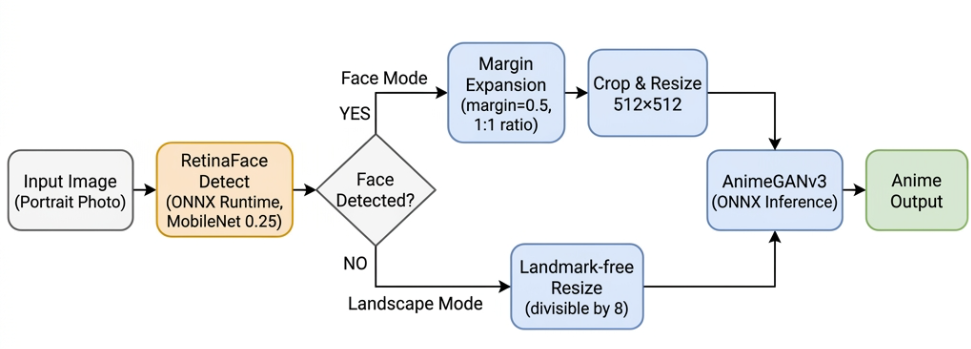
\includegraphics[width=\textwidth]{figChap4/face_extraction_pipeline.png}
    \caption{Pipeline tích hợp Face Extraction vào AnimeGANv3}
    \label{fig:face_extraction_pipeline}
\end{figure}
    \noindent\textit{Chú thích:} Luồng Hybrid (chính): ảnh qua RetinaFace; nếu phát hiện khuôn mặt thì nền chạy Landscape Inference đồng thời mỗi mặt được Margin Expansion $\to$ Crop $512\times512$ $\to$ ONNX Face Inference $\to$ ghép feathered blend; nếu không phát hiện mặt thì toàn bộ ảnh chạy Landscape Inference \cite{Liu2024}.

Kiến trúc này cho phép hệ thống xử lý linh hoạt ba loại kịch bản: ảnh chân dung cận mặt (Face Mode), ảnh phong cảnh (Landscape Mode), và ảnh nhóm người cần giữ cả nền lẫn chất lượng mặt cao (Hybrid Mode). Khi Face Mode hoặc Hybrid Mode được kích hoạt nhưng không phát hiện khuôn mặt nào, hệ thống tự động chuyển sang Landscape Mode --- cơ chế \textbf{hạ cấp mềm} (graceful degradation) đảm bảo hệ thống không bao giờ trả về lỗi cho người dùng.

\medskip
\noindent\textit{\textbf{Phân tích thiết kế:} Việc bổ sung một module tiền xử lý thay vì sửa mô hình sinh ảnh phản ánh một nguyên tắc kỹ thuật mà luận văn cho là đáng lưu ý: \textbf{khi mô hình có một chế độ làm việc tối ưu đã biết, cách rẻ nhất để cải thiện kết quả là đưa dữ liệu về đúng chế độ đó}. DTGAN được huấn luyện trên các mẩu ảnh $256\times256$; mọi đầu vào lệch khỏi phân phối này --- ảnh quá lớn, khuôn mặt quá nhỏ, tỉ lệ khung hình bất thường --- đều khiến mô hình làm việc ngoài vùng thoải mái của nó. Module Face Extraction thực chất là một bộ \textbf{quy chuẩn hóa đầu vào} (input canonicalizer). Đổi lại sự đơn giản đó, hệ thống phải chấp nhận một hệ quả kiến trúc: chất lượng đầu ra giờ đây phụ thuộc vào \textbf{hai} mô hình mắc nối tiếp, và sai sót của bộ phát hiện khuôn mặt sẽ truyền thẳng xuống khâu sinh ảnh mà không có cơ chế nào sửa chữa. Đây là đánh đổi trung tâm của toàn chương và sẽ được đánh giá lại ở Mục~\ref{subsec:pipeline_limitations}.}

% =====================================================
\section{Phát hiện Khuôn mặt với RetinaFace}
\label{sec:retinaface}

\subsection{Tổng quan RetinaFace}
\label{subsec:chap3_retinaface_overview}

RetinaFace \cite{Deng2019RetinaFace} là phương pháp phát hiện khuôn mặt đơn luồng (single-shot) đa tỉ lệ, được công bố tại CVPR 2020. Điểm nổi bật của RetinaFace là thực hiện \textbf{học đa nhiệm} (multi-task learning) đồng thời ba bài toán con trong một lần suy luận: phân loại mặt/không mặt, hồi quy bounding box, và hồi quy 5 điểm đặc trưng khuôn mặt (facial landmarks).

Lợi ích của việc gộp ba nhiệm vụ không chỉ nằm ở tốc độ. Nhiệm vụ hồi quy landmark đóng vai trò \textbf{nhiệm vụ phụ trợ} (auxiliary task): để dự đoán đúng vị trí hai mắt và mũi, mạng buộc phải học biểu diễn nắm bắt được cấu trúc hình học nội tại của khuôn mặt. Biểu diễn đó đồng thời làm cho nhiệm vụ chính --- phân loại và định vị --- trở nên chính xác hơn, đặc biệt với các khuôn mặt bị che khuất một phần hoặc ở góc nghiêng.

Trong hệ thống của luận văn, phiên bản sử dụng backbone \textbf{MobileNet 0.25} \cite{Howard2017MobileNet} --- phiên bản siêu nhẹ của MobileNet chỉ với 25\% số kênh so với MobileNet đầy đủ --- được triển khai thông qua ONNX Runtime \cite{ONNX2019} để đảm bảo tốc độ suy luận cao trên cả CPU lẫn GPU tiêu dùng.

\subsection{Kiến trúc Mạng Phát hiện}
\label{subsec:retinaface_arch}

\begin{figure}[H]
    \centering
    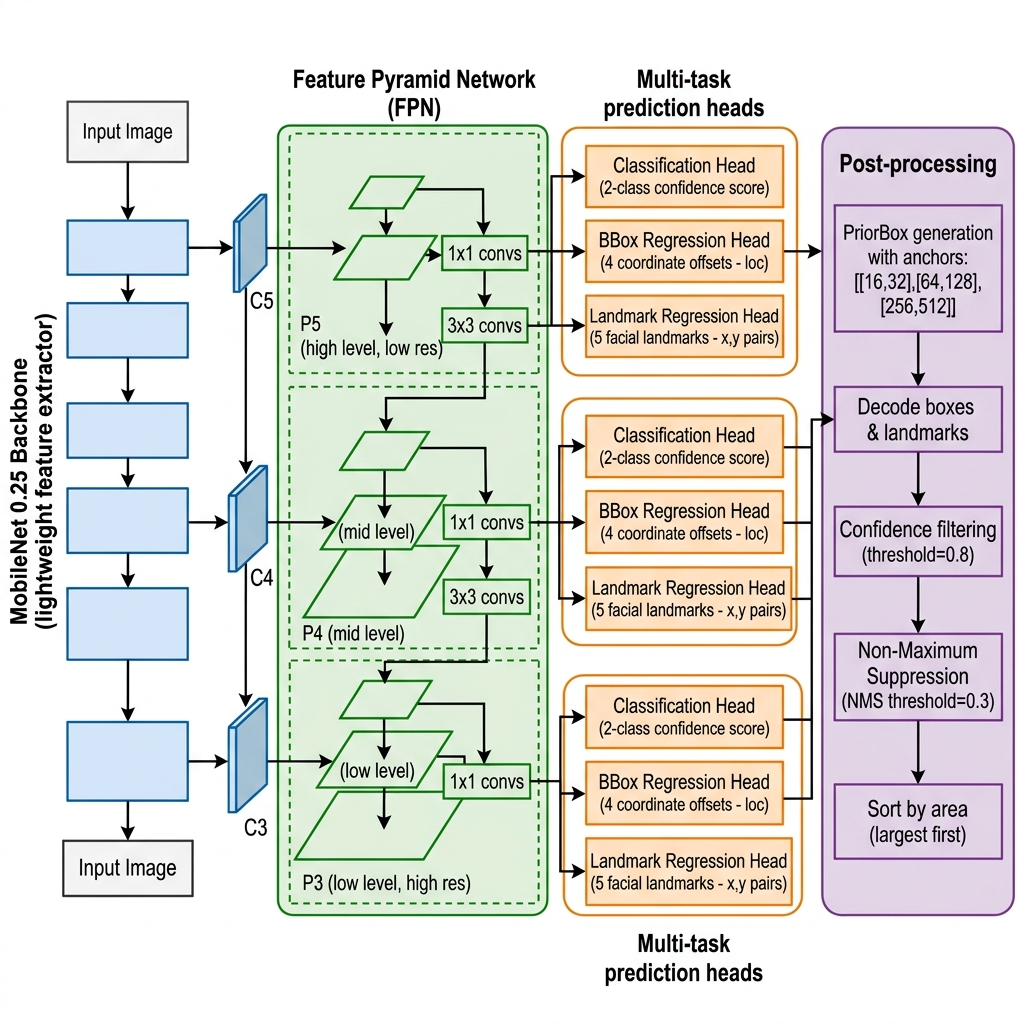
\includegraphics[width=0.95\textwidth]{figChap4/retinaface_architecture.png}
    \caption{Kiến trúc RetinaFace với backbone MobileNet 0.25 và Feature Pyramid Network (FPN)}
    \label{fig:retinaface_arch}
\end{figure}
    \noindent\textit{Chú thích:} Ba đầu ra đa nhiệm tại mỗi cấp FPN: confidence score, bounding box offset (loc), và 5 facial landmarks. Hậu xử lý bao gồm lọc ngưỡng tin cậy (0,8), NMS (0,3), và sắp xếp theo diện tích \cite{Deng2019RetinaFace}

Kiến trúc RetinaFace bao gồm ba thành phần chính:

\subsubsection{Backbone MobileNet 0.25}

MobileNet \cite{Howard2017MobileNet} được thiết kế đặc biệt cho tính toán trên thiết bị nhúng và ứng dụng thời gian thực, sử dụng \textit{depthwise separable convolution} để giảm chi phí tính toán. Ý tưởng là tách một phép tích chập chuẩn thành hai bước: lọc không gian theo từng kênh độc lập (depthwise) rồi trộn kênh bằng tích chập $1\times1$ (pointwise). Tỉ lệ chi phí giữa hai cách làm:

\begin{equation}
\label{eq:depthwise_cost}
\frac{\text{Chi phí depthwise separable}}{\text{Chi phí tích chập chuẩn}}
= \frac{D_K^2 \cdot C_{in} \cdot H W + C_{in} \cdot C_{out} \cdot H W}{D_K^2 \cdot C_{in} \cdot C_{out} \cdot H W}
= \frac{1}{C_{out}} + \frac{1}{D_K^2}
\end{equation}

\noindent trong đó $D_K$ là kích thước kernel, $C_{in}, C_{out}$ là số kênh vào/ra, $H, W$ là kích thước không gian. Với $D_K = 3$ và $C_{out}$ lớn, tỉ lệ này xấp xỉ $1/9$ --- tức tiết kiệm khoảng \textbf{9 lần} chi phí tính toán.

Hệ số nhân chiều rộng (width multiplier) $\alpha = 0{,}25$ thu hẹp thêm số lượng kênh trong mỗi lớp xuống còn 25\%. Vì chi phí tính toán tỉ lệ xấp xỉ bậc hai với số kênh, việc này giảm thêm khoảng $\alpha^2 = 1/16$ chi phí. Kết hợp hai kỹ thuật, backbone đạt kích thước chỉ khoảng 500~KB --- điều kiện tiên quyết để tích hợp vào một ứng dụng web nhẹ.

\subsubsection{Feature Pyramid Network (FPN)}

Feature Pyramid Network \cite{Lin2017FPN} được xây dựng trên các đặc trưng trung gian của backbone để tạo ra biểu diễn đa tỉ lệ $\{P_3, P_4, P_5\}$, cho phép phát hiện khuôn mặt ở nhiều kích thước khác nhau trong cùng một ảnh.

Vấn đề mà FPN giải quyết là một mâu thuẫn cố hữu trong CNN: các tầng nông có độ phân giải cao (tốt cho định vị vật thể nhỏ) nhưng ngữ nghĩa yếu; các tầng sâu có ngữ nghĩa mạnh nhưng độ phân giải thấp. Kiến trúc top-down với các kết nối ngang (lateral connections) truyền ngữ nghĩa từ tầng sâu ngược lên tầng nông:

\begin{equation}
\label{eq:fpn}
P_i = \text{Conv}_{3\times3}\Big( \underbrace{\text{Conv}_{1\times1}(C_i)}_{\text{kết nối ngang}} + \underbrace{\text{Upsample}_{2\times}(P_{i+1})}_{\text{luồng top-down}} \Big)
\end{equation}

\noindent trong đó $C_i$ là đặc trưng tầng thứ $i$ của backbone. Kết quả là mỗi tầng $P_i$ đều mang đồng thời ngữ nghĩa mức cao và độ phân giải không gian phù hợp với dải kích thước mà nó phụ trách.

\subsubsection{Đầu ra Đa nhiệm}

Tại mỗi tầng FPN, ba đầu dự đoán song song được kích hoạt:
\begin{itemize}
    \item \textbf{Classification head:} Xác suất có/không có khuôn mặt tại mỗi anchor.
    \item \textbf{BBox Regression head (\texttt{loc}):} 4 giá trị offset $(dx, dy, dw, dh)$ so với prior box.
    \item \textbf{Landmark Regression head (\texttt{landms}):} 10 giá trị $(x_i, y_i)$ cho 5 điểm đặc trưng: mắt trái, mắt phải, mũi, khóe miệng trái, khóe miệng phải.
\end{itemize}

\subsection{Tiền xử lý Ảnh Đầu vào}
\label{subsec:retinaface_preprocess}

Trước khi đưa vào mạng RetinaFace, ảnh được tiền xử lý theo chuẩn ImageNet:

\begin{enumerate}
    \item Chuyển kiểu dữ liệu sang \texttt{float32}
    \item Trừ giá trị mean ImageNet theo từng kênh:
    \begin{equation}
    \label{eq:imagenet_mean}
    \text{img} \leftarrow \text{img} - (123{,}0;\ 117{,}0;\ 104{,}0)
    \end{equation}
    \item Chuyển thứ tự trục từ $H \times W \times C$ (HWC) sang $C \times H \times W$ (CHW):
    \begin{equation}
    \label{eq:hwc2chw}
    \text{img} = \text{img}^{T}_{(2,0,1)}
    \end{equation}
    \item Mở rộng chiều batch: $\text{img} \in \mathbb{R}^{1 \times C \times H \times W}$
\end{enumerate}

Ba điểm cần lưu ý về bước tiền xử lý này:

\begin{itemize}
    \item \textbf{Chỉ trừ trung bình, không chia độ lệch chuẩn.} Đây là quy ước tiền xử lý của họ mô hình Caffe mà RetinaFace kế thừa, khác với quy ước của PyTorch (chia thêm cho \texttt{std}). Áp dụng sai quy ước sẽ khiến đầu vào lệch thang đo và độ chính xác phát hiện sụt giảm nghiêm trọng --- một lỗi tích hợp phổ biến và khó phát hiện vì mô hình vẫn chạy, chỉ là kết quả kém.
    \item \textbf{Thứ tự kênh BGR.} Bộ ba $(123{,}0;\ 117{,}0;\ 104{,}0)$ tương ứng với thứ tự BGR của OpenCV, không phải RGB. Trong pipeline của luận văn, ảnh được đọc bằng Pillow ở định dạng RGB, nên cần chuyển đổi thứ tự kênh trước khi trừ trung bình.
    \item \textbf{Không resize về kích thước cố định.} Nhờ kiến trúc hoàn toàn tích chập (fully convolutional), RetinaFace chấp nhận ảnh ở kích thước bất kỳ; số lượng prior box được sinh động theo kích thước đầu vào. Đây là lý do bước giới hạn cạnh dài 1280~pixel ở Mục~\ref{subsec:read_resize} lại quan trọng: nó vừa kiểm soát bộ nhớ, vừa kiểm soát số lượng anchor cần hậu xử lý.
\end{itemize}

\subsection{Hậu xử lý và Prior Box}
\label{subsec:retinaface_postprocess}

\subsubsection{Prior Box (Anchor)}

Mô hình sử dụng hệ thống Prior Box đa tỉ lệ với cấu hình \texttt{cfg\_mnet}:

\begin{table}[H]
\caption{Cấu hình Prior Box của RetinaFace với backbone MobileNet 0.25}
\label{tab:prior_box}
\centering
\begin{tabular}{|c|c|c|c|}
\hline
\textbf{Tầng FPN} & \textbf{Stride} & \textbf{Anchor sizes} & \textbf{Đối tượng phát hiện} \\
\hline
$P_3$ (high res) & 8 & $[16, 32]$ px & Khuôn mặt rất nhỏ \\
\hline
$P_4$ & 16 & $[64, 128]$ px & Khuôn mặt nhỏ -- trung bình \\
\hline
$P_5$ (low res) & 32 & $[256, 512]$ px & Khuôn mặt lớn, cận cảnh \\
\hline
\end{tabular}
\end{table}

Prior box (hay anchor) là các khung tham chiếu có kích thước định trước, được rải đều trên lưới không gian của từng tầng FPN. Mạng không dự đoán tọa độ tuyệt đối của khuôn mặt --- một bài toán hồi quy khó với miền giá trị rộng --- mà chỉ dự đoán \textbf{độ lệch tương đối} so với prior box gần nhất. Cách này thu hẹp đáng kể miền đầu ra cần học và giúp mạng hội tụ nhanh hơn.

Tổng số prior box sinh ra cho một ảnh kích thước $H \times W$:

\begin{equation}
\label{eq:num_priors}
N_{\text{prior}} = \sum_{i \in \{3,4,5\}} 2 \cdot \left\lceil \frac{H}{s_i} \right\rceil \cdot \left\lceil \frac{W}{s_i} \right\rceil, \qquad s_i \in \{8, 16, 32\}
\end{equation}

\noindent với hệ số 2 tương ứng hai kích thước anchor tại mỗi tầng. Với ảnh $1280 \times 960$, con số này xấp xỉ $50.000$ prior box --- lý giải vì sao các bước lọc ở phần sau lại cần thiết đến vậy.

\textbf{Nhận xét về dải kích thước.} Bảng~\ref{tab:prior_box} cho thấy các anchor phủ dải từ 16 đến 512~pixel. Tầng $P_3$ với anchor 16~px về lý thuyết cho phép phát hiện khuôn mặt rất nhỏ; tuy nhiên, như kết quả thực nghiệm ở Chương~4 chỉ ra, độ chính xác thực tế với khuôn mặt dưới $32\times32$~px giảm còn khoảng 71\% precision. Nguyên nhân không nằm ở thiết kế anchor mà ở dung lượng biểu diễn của backbone MobileNet~0.25: với chỉ 25\% số kênh, các tầng nông đơn giản không đủ khả năng phân biệt một khuôn mặt 16~pixel với các mẫu nhiễu có cấu trúc tương tự.

\subsubsection{Giải mã Kết quả}

Từ output thô của mạng, bounding boxes và landmarks được giải mã từ offset tương đối sang tọa độ tuyệt đối:

\begin{equation}
\label{eq:decode_box}
\hat{b}_x = p_x + \text{loc}_x \cdot \text{var}_0 \cdot p_w, \quad
\hat{b}_y = p_y + \text{loc}_y \cdot \text{var}_0 \cdot p_h
\end{equation}
\begin{equation}
\label{eq:decode_box2}
\hat{b}_w = p_w \cdot e^{\,\text{loc}_w \cdot \text{var}_1}, \quad
\hat{b}_h = p_h \cdot e^{\,\text{loc}_h \cdot \text{var}_1}
\end{equation}

\noindent trong đó:
\begin{itemize}
    \item $(p_x, p_y, p_w, p_h)$ --- tọa độ tâm và kích thước của prior box, đã chuẩn hóa về $[0,1]$ theo kích thước ảnh.
    \item $(\text{loc}_x, \text{loc}_y, \text{loc}_w, \text{loc}_h)$ --- bốn giá trị thô do mạng dự đoán.
    \item $(\text{var}_0, \text{var}_1) = (0{,}1;\ 0{,}2)$ --- các tham số phương sai, đóng vai trò hệ số tỉ lệ cố định.
\end{itemize}

\textbf{Ý nghĩa của hai dạng công thức khác nhau:}
\begin{itemize}
    \item \textbf{Tọa độ tâm (Phương trình~\ref{eq:decode_box}) dùng dịch chuyển tuyến tính}, và độ dịch được nhân với $p_w$ (hoặc $p_h$). Điều này khiến sai số dự đoán được đo \textit{theo tỉ lệ kích thước khuôn mặt} chứ không theo pixel tuyệt đối: lệch 5~pixel trên một khuôn mặt 500~px là không đáng kể, nhưng trên khuôn mặt 20~px lại là sai lầm lớn. Cách tham số hóa này đảm bảo mạng đối xử công bằng với mọi kích thước khuôn mặt.
    \item \textbf{Kích thước (Phương trình~\ref{eq:decode_box2}) dùng hàm mũ.} Có hai lý do. Thứ nhất, hàm mũ luôn cho kết quả dương, nên chiều rộng và chiều cao dự đoán không bao giờ âm --- mạng không cần học ràng buộc này. Thứ hai, hàm mũ biến phép \textit{nhân} tỉ lệ thành phép \textit{cộng} trong không gian dự đoán: $\text{loc}_w = 0$ nghĩa là giữ nguyên kích thước anchor, $\text{loc}_w > 0$ là phóng to, $\text{loc}_w < 0$ là thu nhỏ, và mức độ thay đổi đối xứng theo tỉ lệ.
    \item \textbf{Vai trò của $\text{var}_0, \text{var}_1$.} Hai hằng số này chuẩn hóa thang đo của đầu ra hồi quy về vùng lân cận 0 với độ lớn tương đương nhau, giúp bốn thành phần của $\text{loc}$ đóng góp cân bằng vào hàm mất mát khi huấn luyện. Giá trị $\text{var}_1 = 0{,}2 > \text{var}_0 = 0{,}1$ phản ánh thực tế rằng sai số về kích thước thường lớn hơn sai số về vị trí tâm.
\end{itemize}

Năm điểm landmark được giải mã theo cùng nguyên tắc như tọa độ tâm:
\begin{equation}
\label{eq:decode_landmark}
\hat{\ell}_x^{(k)} = p_x + \text{landms}_x^{(k)} \cdot \text{var}_0 \cdot p_w, \qquad k = 1, \dots, 5
\end{equation}

\subsubsection{Lọc và Non-Maximum Suppression}

Quá trình hậu xử lý gồm 5 bước tuần tự, thu gọn từ hàng chục nghìn ứng viên xuống tối đa 5 khuôn mặt:

\begin{enumerate}
    \item \textbf{Lọc ngưỡng tin cậy:} Chỉ giữ các detection có confidence $> 0{,}8$ (tham số \texttt{confidence\_threshold}).
    \item \textbf{Giữ Top-K trước NMS:} Sắp xếp theo confidence giảm dần, chỉ giữ tối đa $K_1 = 10$ detection có điểm cao nhất (tham số \texttt{top\_k}) nhằm giảm chi phí tính toán NMS.
    \item \textbf{Non-Maximum Suppression (NMS):} Loại bỏ các bounding box trùng lặp với $\text{IoU} > 0{,}3$ (tham số \texttt{nms\_threshold}).
    \item \textbf{Giữ Top-K sau NMS:} Chỉ giữ tối đa $K_2 = 5$ khuôn mặt (tham số \texttt{keep\_top\_k}).
    \item \textbf{Sắp xếp theo diện tích:} Khuôn mặt lớn nhất (chủ thể chính) được đặt lên đầu danh sách:
    \begin{equation}
    \label{eq:sort_area}
    \text{order} = \text{argsort}\!\left[(x_2 - x_1)(y_2 - y_1)\right]_{\text{giảm dần}}
    \end{equation}
\end{enumerate}

\textbf{Vì sao cần NMS.} Do prior box được rải dày đặc, một khuôn mặt duy nhất thường kích hoạt hàng chục anchor lân cận, tạo ra nhiều bounding box gần trùng nhau. NMS giải quyết bằng thuật toán tham lam: chọn box có điểm cao nhất, loại bỏ mọi box chồng lấp quá ngưỡng với nó, rồi lặp lại trên phần còn lại. Độ chồng lấp được đo bằng hệ số IoU (Intersection over Union):

\begin{equation}
\label{eq:iou}
\text{IoU}(B_1, B_2) = \frac{|B_1 \cap B_2|}{|B_1 \cup B_2|} = \frac{\text{diện tích phần giao}}{\text{diện tích phần hợp}} \in [0, 1]
\end{equation}

\textbf{Ý nghĩa của các ngưỡng đã chọn.} Bộ tham số $(0{,}8;\ 0{,}3;\ 10;\ 5)$ phản ánh rõ một triết lý: \textbf{ưu tiên độ chính xác hơn độ bao phủ}.

\begin{itemize}
    \item \textbf{Ngưỡng tin cậy $0{,}8$} là mức khá cao (nhiều hệ thống dùng $0{,}5$). Lựa chọn này chấp nhận bỏ sót một số khuôn mặt để gần như loại trừ khả năng phát hiện nhầm. Lý do nằm ở hậu quả bất đối xứng của hai loại lỗi: bỏ sót khuôn mặt chỉ khiến hệ thống hạ cấp về Landscape Mode --- kết quả vẫn chấp nhận được; ngược lại, phát hiện nhầm sẽ khiến một vùng nền ngẫu nhiên bị anime hóa như khuôn mặt rồi ghép đè lên ảnh, tạo ra lỗi thị giác rõ rệt.
    \item \textbf{Ngưỡng NMS $0{,}3$} nghiêm ngặt hơn mức thông thường ($0{,}5$), nghĩa là hai box chỉ cần chồng lấp 30\% đã bị coi là trùng. Đây là lựa chọn phù hợp với bài toán ảnh chân dung, nơi các khuôn mặt hiếm khi che khuất nhau nhiều. Tuy nhiên, cần ghi nhận rằng ngưỡng này sẽ gây bỏ sót trong ảnh nhóm đông người đứng sát nhau --- một hạn chế đã biết của thiết kế.
    \item \textbf{Giới hạn $K_2 = 5$ khuôn mặt} được đặt ra chủ yếu vì lý do hiệu năng của Hybrid Mode: mỗi khuôn mặt phát sinh thêm một lần suy luận ONNX (xem Mục~\ref{subsec:hybrid_complexity}).
\end{itemize}

Trong chế độ Face Mode, phần tử đầu tiên (\texttt{bboxes[0]}) --- khuôn mặt lớn nhất --- được chọn làm đối tượng chuyển đổi. Trong chế độ Hybrid Mode, toàn bộ danh sách khuôn mặt sau lọc đều được xử lý. Nếu kết quả rỗng, hàm trả về \texttt{None} và pipeline chuyển sang Landscape Mode.

\medskip
\noindent\textit{\textbf{Nhận xét:} Việc sắp xếp theo \textbf{diện tích} thay vì theo \textbf{điểm tin cậy} ở bước 5 là một chi tiết nhỏ nhưng phản ánh đúng ngữ nghĩa bài toán. Điểm tin cậy trả lời câu hỏi ``\textit{đây có phải khuôn mặt không?}'', trong khi thứ hệ thống cần biết là ``\textit{đâu là khuôn mặt mà người dùng quan tâm?}''. Trong nhiếp ảnh chân dung, chủ thể chính hầu như luôn là khuôn mặt lớn nhất khung hình --- một quy ước bố cục ổn định đến mức có thể dùng làm heuristic đáng tin cậy. Dù vậy, cần thừa nhận rằng heuristic này thất bại trong một số tình huống thực tế: ảnh có người đứng gần camera nhưng không phải chủ thể (người qua đường lọt khung), hoặc ảnh nhóm mà chủ thể đứng ở hàng sau. Với những trường hợp đó, Hybrid Mode --- xử lý toàn bộ khuôn mặt --- là lời giải đúng đắn hơn, và đây chính là một trong những động lực dẫn tới việc luận văn bổ sung chế độ này.}

% =====================================================
\section{Kỹ thuật Mở rộng Vùng Khuôn mặt (Margin Expansion)}
\label{sec:margin_expansion}

\subsection{Động lực và Mục tiêu}
\label{subsec:margin_motivation}

Bounding box khuôn mặt trả về bởi RetinaFace thường chỉ bao quanh phần khuôn mặt thuần túy (từ trán đến cằm, từ tai này đến tai kia). Nếu cắt đúng theo bounding box này để đưa vào mô hình AnimeGANv3, ảnh đầu ra sẽ thiếu ngữ cảnh quan trọng: tóc, cổ, vai --- những thành phần không thể thiếu để tạo ra ảnh anime chân dung trông tự nhiên và hoàn chỉnh.

Vấn đề còn nghiêm trọng hơn ở khía cạnh phân phối dữ liệu. Tập ảnh huấn luyện của DTGAN gồm các ảnh chân dung thông thường, trong đó khuôn mặt luôn xuất hiện cùng tóc và nền. Một mẩu ảnh chỉ chứa da mặt là đầu vào \textbf{ngoài phân phối huấn luyện} (out-of-distribution) --- mô hình chưa từng gặp dạng dữ liệu này và không có cơ sở để xử lý đúng.

Kỹ thuật \textbf{Adaptive Gaze-Dependent Margin Expansion} (AGME --- mở rộng lề thích nghi theo hướng nhìn) được phát triển trong luận văn nhằm ba mục tiêu đồng thời:
\begin{enumerate}
    \item Mở rộng bounding box theo tỉ lệ phần trăm kích thước mặt, đảm bảo bao phủ đủ ngữ cảnh.
    \item Duy trì tỉ lệ khung hình 1:1 (vuông), phù hợp với yêu cầu đầu vào $512 \times 512$ của mô hình --- tránh biến dạng hình học do resize không đồng đều hai chiều.
    \item Phân bổ \textit{ngân sách ngữ cảnh hữu hạn} về đúng nơi phần đầu bị thiếu, thay vì rải đều bốn phía.
\end{enumerate}

\textbf{Vì sao mở rộng đối xứng là chưa đủ.} Cách làm thông thường --- nới đều một tỉ lệ $m$ ra bốn phía rồi ép vuông --- chỉ tối ưu dưới hai giả định ngầm: khuôn mặt chính diện, và khuôn mặt nằm giữa box theo chiều dọc. Cả hai đều thường xuyên bị vi phạm. RetinaFace, giống phần lớn bộ phát hiện một giai đoạn, hồi quy một box ôm sát \textit{bề mặt khuôn mặt nhìn thấy được}: vùng trải từ lông mày, mắt, mũi tới miệng. Từ đó sinh ra hai thiên lệch có hệ thống:

\begin{itemize}
    \item \textbf{Thiên lệch ngang do góc xoay (yaw).} Khi đối tượng quay sang trái ảnh, vùng chẩm --- phía sau hộp sọ, tai và khối tóc --- nhô ra phía \textit{phải} ảnh, nằm khá xa ngoài box; trong khi ở phía trái, box đã sát mép bóng đầu. Mở rộng đối xứng vì thế tiêu một nửa ngân sách vào nền ở phía nhìn, mà vẫn cắt cụt khối tóc ở phía đối diện. Tăng $m$ để bù không giải quyết được vấn đề: nó nạp thêm nền vào \textit{cả hai} phía.
    \item \textbf{Thiên lệch dọc không có trung bình bằng không.} Trán, đỉnh đầu và khối tóc phía trên đường lông mày luôn lớn hơn phần cằm--cổ phía dưới miệng, nên chia đôi đều theo chiều dọc sẽ cắt mất đỉnh đầu trong khi lãng phí các hàng pixel vào cổ áo.
\end{itemize}

Luận văn vì vậy \textbf{giữ nguyên tổng ngân sách ngang ở mức $2m \cdot w$} và chỉ \textit{phân bổ lại} nó theo tư thế đầu quan sát được.

\begin{figure}[H]
    \centering
    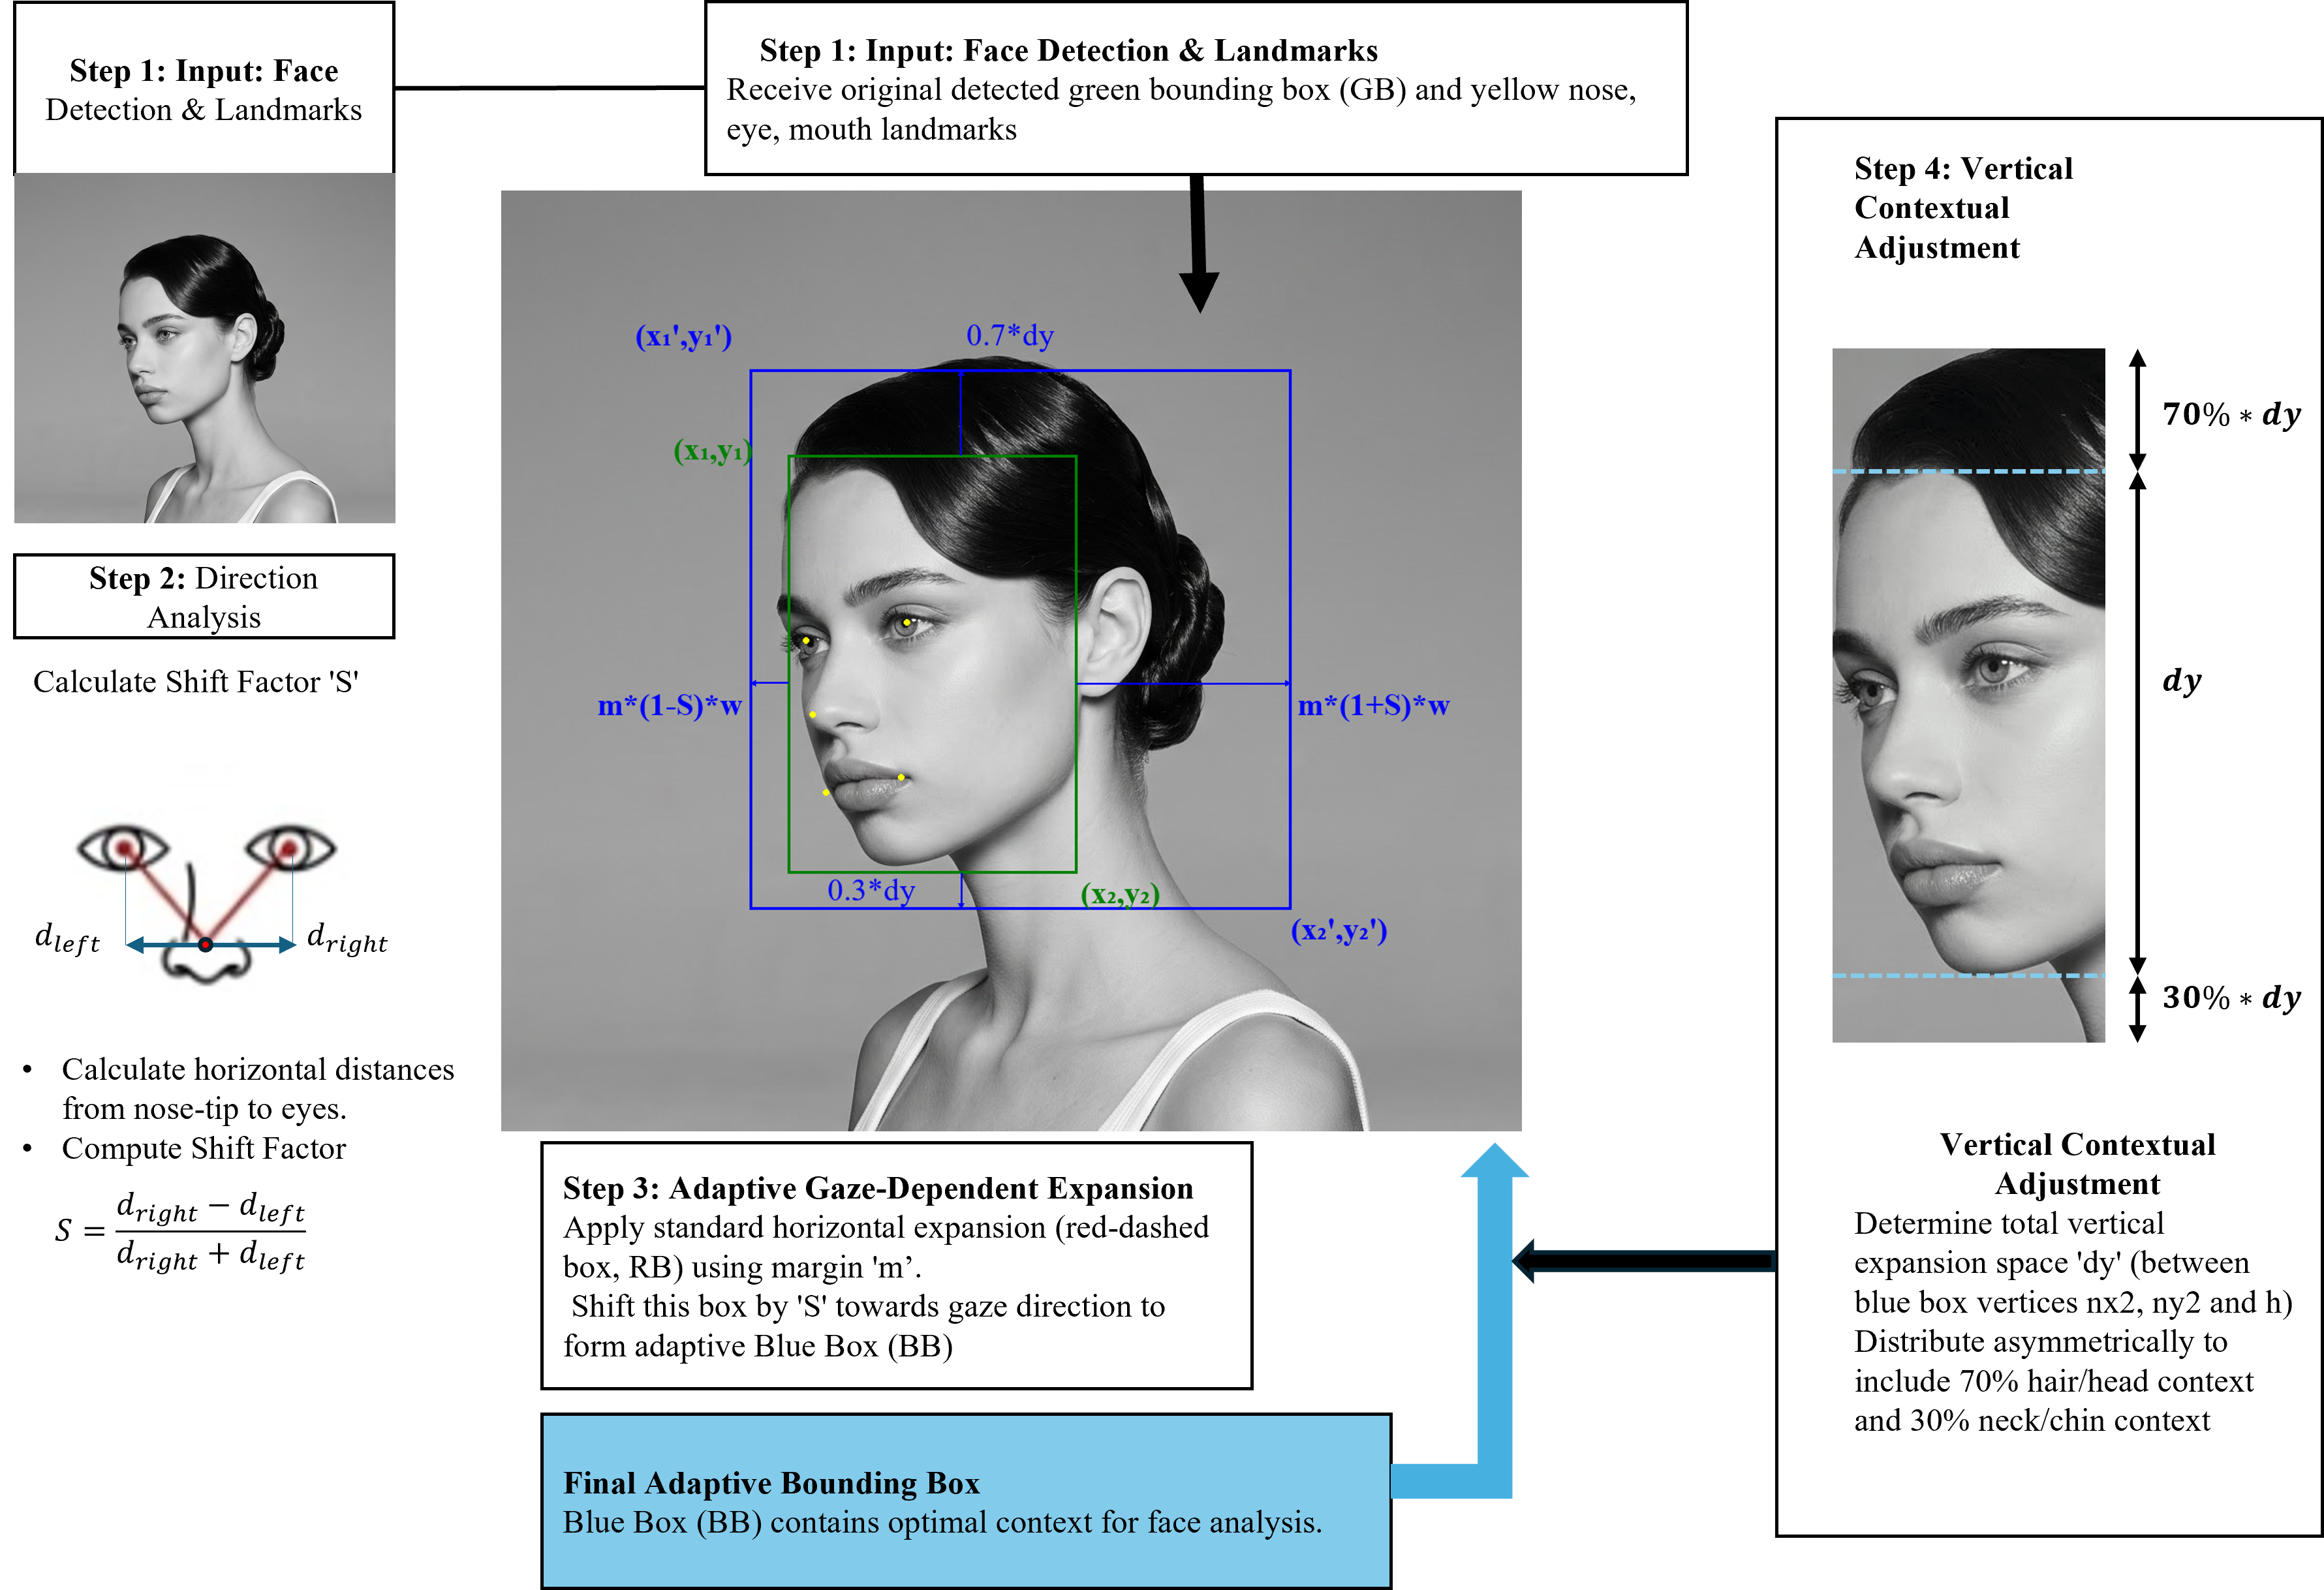
\includegraphics[width=0.85\textwidth]{figChap4/adaptive_margin_pipeline.png}
    \caption{Minh họa kỹ thuật Margin Expansion}
    \label{fig:margin_expansion}
\end{figure}
    \noindent\textit{Chú thích:} Bounding box gốc (nét xanh lá) cùng năm điểm landmark (vàng) được dùng để ước lượng hệ số dịch chuyển $S$; ngân sách ngang cố định $2m\,w$ được tách thành $m(1-S)w$ bên trái và $m(1+S)w$ bên phải, dịch phần mở rộng về phía sau gáy. Ràng buộc vuông sinh ra phần dư thừa dọc $dy$, chia $70\%$ lên đỉnh đầu và $30\%$ xuống cằm, cho vùng cắt thích nghi (nét xanh dương).

\subsection{Thuật toán Margin Expansion}
\label{subsec:margin_algorithm}

Cho bounding box khuôn mặt $(x_1, y_1, x_2, y_2)$, tập năm điểm landmark $L = \{\mathbf{p}_{e_1}, \mathbf{p}_{e_2}, \mathbf{p}_{n}, \mathbf{p}_{m_1}, \mathbf{p}_{m_2}\}$ (hai tâm mắt, đỉnh mũi, hai khóe miệng), kích thước ảnh $(H, W)$ và hệ số mở rộng cơ sở $m = 0{,}3$, thuật toán thực hiện theo 6 bước.

\textbf{Bước 1 --- Thang tham chiếu.} Bề rộng tham chiếu được lấy là cạnh \textit{lớn hơn} trong hai cạnh của box:
\begin{equation}
\label{eq:margin_step1}
w = \max\big(x_2 - x_1,\; y_2 - y_1\big), \qquad h = y_2 - y_1
\end{equation}

Việc dùng $\max(\cdot)$ thay vì $x_2 - x_1$ là có chủ đích. Ở góc xoay lớn, box phát hiện được hẹp lại --- khoảng cách hai mắt trong phép chiếu co theo $\cos\theta$ --- nên một lề neo theo bề rộng sẽ teo đi \textit{đúng lúc} cần thêm ngữ cảnh. Neo vào cạnh trội giữ cho lượng ngữ cảnh tuyệt đối ổn định qua các tư thế.

\textbf{Bước 2 --- Hệ số dịch chuyển theo hướng nhìn.} Gọi $x_\ell = \min(x_{e_1}, x_{e_2})$ và $x_r = \max(x_{e_1}, x_{e_2})$ là hoành độ mắt phía trái và phía phải ảnh. Hai khoảng cách mũi--mắt theo trục ngang:
\begin{equation}
\label{eq:margin_dlr}
d_{\text{left}} = \max\big(1,\; x_n - x_\ell\big), \qquad d_{\text{right}} = \max\big(1,\; x_r - x_n\big)
\end{equation}
trong đó phép chặn tại 1~pixel ngăn chia cho 0 ở các góc nhìn gần như nghiêng hoàn toàn. Độ bất đối xứng đã chuẩn hóa:
\begin{equation}
\label{eq:margin_shift}
S = \operatorname{clip}\!\left(\frac{d_{\text{right}} - d_{\text{left}}}{d_{\text{right}} + d_{\text{left}}},\ -S_{\max},\ S_{\max}\right), \qquad S_{\max} = 0{,}7
\end{equation}

Đại lượng $S$ không thứ nguyên và bất biến theo tỉ lệ, đóng vai trò một \textit{proxy} cho góc xoay: $S = 0$ với mặt chính diện, $S > 0$ khi đầu quay sang trái ảnh (mũi tiến lại gần mắt trái trong phép chiếu nên $d_{\text{left}}$ co lại), và $S < 0$ cho trường hợp đối xứng gương. Chặn $S_{\max} = 0{,}7$ ngăn một khuôn mặt gần như nghiêng hoàn toàn --- hoặc một landmark ngoại lai --- dịch vùng cắt xa tới mức chính khuôn mặt trôi ra biên.

\textbf{Bước 3 --- Mở rộng ngang bất đối xứng.} Tỉ lệ lề hai phía:
\begin{equation}
\label{eq:margin_msplit}
m_{\text{left}} = m\,(1 - S), \qquad m_{\text{right}} = m\,(1 + S)
\end{equation}
\begin{equation}
\label{eq:margin_step2}
x_1' = \max\big(0,\; x_1 - m_{\text{left}}\, w\big), \qquad x_2' = \min\big(W,\; x_2 + m_{\text{right}}\, w\big)
\end{equation}

Vì $m_{\text{left}} + m_{\text{right}} = 2m$ với mọi $S$, tổng ngữ cảnh ngang được \textbf{bảo toàn}: AGME không bao giờ làm vùng cắt lớn hơn so với mở rộng đối xứng, nó chỉ dịch phần dư thừa sang phía sau gáy. Đây chính là điều cho phép hệ thống bền vững hơn với tư thế mà không phải trả giá bằng nhiễu nền của một $m$ lớn hơn.

\textbf{Bước 4 --- Ép tỉ lệ 1:1:}
\begin{equation}
\label{eq:margin_step4}
w' = x_2' - x_1', \qquad h' = w'
\end{equation}

\textbf{Bước 5 --- Phân bổ dọc bất đối xứng.} Ràng buộc vuông sinh ra phần dư thừa theo chiều dọc:
\begin{equation}
\label{eq:margin_step5}
dy = h' - h = (x_2' - x_1') - h
\end{equation}

Ở chế độ thường $dy \geq 0$, phần dư thừa được chia theo hệ số ưu tiên đỉnh đầu $\alpha_{\text{top}}$:
\begin{align}
\label{eq:margin_step5b}
y_1' &= \max\big(0,\; y_1 - \alpha_{\text{top}}\, dy\big) \\
y_2' &= \min\big(H,\; y_2 + (1 - \alpha_{\text{top}})\, dy\big)
\end{align}
với $\alpha_{\text{top}} = 0{,}7$ khi có landmarks và $\alpha_{\text{top}} = 0{,}5$ khi không có. Tỉ lệ $70{:}30$ phản ánh tiên nghiệm giải phẫu đã nêu: chân tóc và đỉnh đầu mang nhiều tín hiệu nhận dạng lẫn tín hiệu phong cách cho việc dựng ảnh anime hơn hẳn phần cổ và cổ áo.

Ở chế độ suy biến $dy < 0$ --- box rộng hơn cao, thường do bị chặn cứng ở biên ngang --- phần chiều cao thừa được cắt bớt đối xứng:
\begin{align}
\label{eq:margin_step5d}
y_1' &= \max\big(0,\; y_1 + |dy|/2\big) \\
y_2' &= \min\big(H,\; y_2 - |dy|/2\big)
\end{align}

\textbf{Bước 6 --- Làm tròn về chỉ số nguyên:} vùng cắt cuối cùng là $B' = \big(\lfloor x_1' \rfloor, \lfloor y_1' \rfloor, \lfloor x_2' \rfloor, \lfloor y_2' \rfloor\big)$, dùng trực tiếp làm chỉ số cắt mảng.

\begin{algorithm}[H]
\caption{Adaptive Gaze-Dependent Margin Expansion (AGME)}
\label{alg:margin_expansion}
\begin{algorithmic}[1]
\Require Bounding box $(x_1, y_1, x_2, y_2)$; kích thước ảnh $(H, W)$; hệ số $m = 0{,}3$; landmarks $L$ (tùy chọn); chặn $S_{\max} = 0{,}7$
\Ensure Vùng cắt vuông thích nghi $(x_1', y_1', x_2', y_2')$ nằm trọn trong ảnh
\State $w \gets \max(x_2 - x_1,\ y_2 - y_1)$;\quad $h \gets y_2 - y_1$ \Comment{Bước 1}
\State $m_{\text{left}} \gets m$;\quad $m_{\text{right}} \gets m$;\quad $\alpha_{\text{top}} \gets 0{,}5$
\If{$L \neq \varnothing$} \Comment{Bước 2}
    \State $x_\ell \gets \min(x_{e_1}, x_{e_2})$;\quad $x_r \gets \max(x_{e_1}, x_{e_2})$
    \State $d_{\text{left}} \gets \max(1,\ x_n - x_\ell)$;\quad $d_{\text{right}} \gets \max(1,\ x_r - x_n)$
    \State $S \gets (d_{\text{right}} - d_{\text{left}}) / (d_{\text{right}} + d_{\text{left}})$
    \State $S \gets \operatorname{clip}(S,\ -S_{\max},\ S_{\max})$
    \State $m_{\text{left}} \gets m(1 - S)$;\quad $m_{\text{right}} \gets m(1 + S)$ \Comment{Bước 3}
    \State $\alpha_{\text{top}} \gets 0{,}7$ \Comment{ưu tiên đỉnh đầu}
\EndIf
\State $x_1' \gets \max(0,\ x_1 - m_{\text{left}}\,w)$;\quad $x_2' \gets \min(W,\ x_2 + m_{\text{right}}\,w)$
\State $w' \gets x_2' - x_1'$;\quad $h' \gets w'$ \Comment{Bước 4: ép tỉ lệ 1:1}
\State $dy \gets h' - h$ \Comment{Bước 5}
\If{$dy \geq 0$}
    \State $y_1' \gets \max(0,\ y_1 - \alpha_{\text{top}}\, dy)$
    \State $y_2' \gets \min(H,\ y_2 + (1 - \alpha_{\text{top}})\, dy)$
\Else
    \State $y_1' \gets \max(0,\ y_1 + |dy|/2)$;\quad $y_2' \gets \min(H,\ y_2 - |dy|/2)$
\EndIf
\State \Return $\big(\lfloor x_1' \rfloor,\ \lfloor y_1' \rfloor,\ \lfloor x_2' \rfloor,\ \lfloor y_2' \rfloor\big)$ \Comment{Bước 6}
\end{algorithmic}
\end{algorithm}

\textbf{Vì sao bảo toàn ngân sách lại quan trọng hơn là nới rộng ngân sách.} Cách xử lý trực giác cho vấn đề cắt cụt tóc ở tư thế nghiêng là tăng $m$. Nhưng $m$ tác động lên \textit{cả hai} phía, nên nó nạp thêm nền ở phía nhìn --- nơi vốn đã thừa --- để mua thêm một chút tóc ở phía sau gáy. Kết cục là kết cấu ngoài miền (off-domain) tăng lên ở cả hai phía, đúng loại nhiễu mà các cơ chế thống kê toàn cục của DTGAN (LADE, External Attention --- Chương~2, Mục~\ref{subsec:ext_attention_arch}) nhạy cảm nhất. Công thức~(\ref{eq:margin_msplit}) tách bạch hai đại lượng vốn bị gộp làm một trong mở rộng đối xứng: \textit{lượng} ngữ cảnh do $m$ quyết định, còn \textit{vị trí} đặt ngữ cảnh đó do $S$ quyết định. Nhờ vậy có thể sửa lỗi phân bổ mà không phải đụng tới lượng.

\subsection{Tính chất của thuật toán}
\label{subsec:margin_properties}

Từ các công thức trên có thể rút ra ba tính chất định lượng hữu ích cho việc phân tích ở các mục sau:

\textbf{Tính chất 1 --- Bề rộng vùng cắt.} Gọi $w_{\text{box}} = x_2 - x_1$ là bề rộng box gốc và $r = w / w_{\text{box}} \geq 1$ là tỉ số giữa thang tham chiếu và bề rộng box. Khi không bị chặn biên:
\begin{equation}
\label{eq:crop_width}
w' = w_{\text{box}} + 2 m w = \big(1 + 2 m r\big)\, w_{\text{box}}
\end{equation}

Với box vuông ($r = 1$) và $m = 0{,}3$, vùng cắt rộng gấp $1{,}6$ lần box gốc. Trên tập đánh giá, tỉ lệ khung hình trung bình của box RetinaFace là $h / w_{\text{box}} \approx 1{,}32$, nên $\max(\cdot)$ thường trả về chiều cao và $r \approx 1{,}32$: mỗi phía giữ được khoảng $m r \approx 0{,}4\, w_{\text{box}}$ ngữ cảnh, đưa vùng cắt lên khoảng $1{,}8$ lần box gốc.

\medskip
\noindent\textit{Lưu ý về khả năng so sánh:} vì thang tham chiếu là $\max(\cdot)$ chứ không phải bề rộng, giá trị $m$ ở đây \textbf{không cùng đơn vị} với $m$ của mở rộng đối xứng neo theo bề rộng. Cùng một con số danh nghĩa, công thức này mua nhiều hơn khoảng $1{,}3$ lần lượng đệm tuyệt đối, nên điểm tối ưu dịch xuống: $m = 0{,}3$ ở đây tương đương khoảng $m \approx 0{,}5$ của công thức neo theo bề rộng. Hai giá trị mô tả những vùng cắt tương đương, không phải một sự cắt giảm ngữ cảnh.

\textbf{Tính chất 2 --- Vùng cắt vuông không được bảo đảm tuyệt đối.} Bước 4 đặt $h' = w'$, nhưng Bước 5 lại áp thêm các toán tử $\max(0,\cdot)$ và $\min(H,\cdot)$. Nếu khuôn mặt nằm gần biên trên hoặc biên dưới, chiều cao thực tế sẽ nhỏ hơn $h'$ và vùng cắt trở thành hình chữ nhật. Khi đó, phép \texttt{resize} về $512\times512$ sẽ gây biến dạng tỉ lệ khung hình. Đây là một hạn chế đã biết của cài đặt hiện tại; hướng khắc phục là đệm thêm viền (padding) thay vì cắt cụt, sẽ được bàn ở Mục~\ref{subsec:pipeline_limitations}.

\textbf{Tính chất 3 --- Bề rộng khuôn mặt sau chuẩn hóa nằm trong một dải hẹp.} Kết hợp Tính chất 1 với bước resize về $512\times512$, khuôn mặt trong ảnh đưa vào Generator có bề rộng:
\begin{equation}
\label{eq:face_width_after}
w_{\text{model}} = 512 \cdot \frac{w_{\text{box}}}{w'} = \frac{512}{1 + 2 m r}
\end{equation}

\noindent \textit{không phụ thuộc vào kích thước khuôn mặt trong ảnh gốc}, mà chỉ phụ thuộc tỉ lệ khung hình của box qua $r$. Với $m = 0{,}3$:
\begin{itemize}
    \item $r = 1$ (box vuông): $w_{\text{model}} = 320$~pixel --- cận trên.
    \item $r \approx 1{,}32$ (giá trị điển hình): $w_{\text{model}} \approx 286$~pixel.
    \item $r = 1{,}67$: $w_{\text{model}} = 256$~pixel.
\end{itemize}

Nói cách khác, chừng nào $h / w_{\text{box}} \leq 1{,}67$ --- đúng với gần như mọi box chân dung --- khuôn mặt luôn được đưa vào Generator ở bề rộng \textbf{ít nhất 256~pixel}, điển hình khoảng \textbf{286~pixel}. Đây là tính chất quan trọng nhất của toàn bộ module: nó biến một đầu vào có kích thước tùy ý thành một đầu vào đã được chuẩn hóa, và sẽ là cơ sở cho phân tích ở Mục~\ref{sec:effective_resolution}. So với công thức neo theo bề rộng, việc thay hằng số bằng một dải hẹp là cái giá phải trả để lượng ngữ cảnh tuyệt đối không bị co lại ở các tư thế nghiêng --- đánh đổi có lợi, vì chính nhóm ảnh nghiêng mới là nhóm khó nhất.

\subsection{Xử lý Trường hợp Đặc biệt (Edge Cases)}
\label{subsec:edge_cases}

Các phép chặn ở Bước 3 và Bước 5, cùng nhánh suy biến $dy < 0$, là cơ chế xử lý edge case:

\begin{itemize}
    \item \textbf{Landmarks không khả dụng:} Khi bộ phát hiện không trả về landmark, thuật toán rơi về $S = 0$ và $\alpha_{\text{top}} = 0{,}5$ --- tức đúng hành vi của mở rộng đối xứng. AGME vì thế là một \textit{mở rộng ngược tương thích}, không phải một nhánh riêng cần bảo trì song song.
    \item \textbf{Khuôn mặt gần biên ảnh:} Toán tử $\max(0,\cdot)$ và $\min(W,\cdot)$ ở Phương trình~(\ref{eq:margin_step2}) chặn vùng cắt lại trong ảnh. Hệ quả là ngân sách ngang không còn được bảo toàn ở phía bị chặn, và vùng cắt lệch khỏi hình vuông đúng bằng lượng bị chặn; phần chênh này được phép resize LANCZOS hấp thụ mà không gây biến dạng nhận thấy được.
    \item \textbf{Khuôn mặt ở góc ảnh:} Cả ràng buộc ngang lẫn dọc cùng có hiệu lực; vùng cắt thu về phần hợp lệ lớn nhất có thể.
    \item \textbf{Khuôn mặt rất lớn (gần bằng ảnh):} Lề bị giới hạn bởi khoảng cách tới biên, vùng cắt gần như trùng với bounding box gốc. Trường hợp này không gây lỗi nhưng cũng không mang lại lợi ích của Margin Expansion.
    \item \textbf{Nhánh suy biến $dy < 0$:} Xảy ra khi lề ngang bị chặn mạnh khiến $w'$ (và do đó $h' = w'$) nhỏ hơn chiều cao khuôn mặt. Thuật toán \textit{cắt bớt} theo chiều dọc, đối xứng hai đầu. Trong nhánh này, hai toán tử $\max(0,\cdot)$ và $\min(H,\cdot)$ ở Phương trình~(\ref{eq:margin_step5d}) là dư thừa về mặt logic --- do $y_1' > y_1 \geq 0$ và $y_2' < y_2 \leq H$ --- nhưng được giữ lại như một lớp bảo vệ phòng thủ chống lại bounding box không hợp lệ.
    \item \textbf{Vùng cắt suy biến:} Với các box rất nhỏ hoặc bị chặn ở cả hai phía, phép làm tròn ở Bước 6 về lý thuyết có thể sinh ra vùng cắt có bề rộng hoặc chiều cao bằng 0. Cài đặt vì vậy ép $x_2' \geq x_1' + 1$ và $y_2' \geq y_1' + 1$ trước khi trả về; ở tầng pipeline, khuôn mặt có cạnh nhỏ hơn 16~pixel còn bị bỏ qua hoàn toàn (Thuật toán~\ref{alg:hybrid_mode}).
\end{itemize}

\subsection{Ý nghĩa của Tham số $m = 0{,}3$}
\label{subsec:margin_value}

Giá trị $m = 0{,}3$ được lựa chọn qua thực nghiệm (kết quả định lượng trình bày tại Mục~\ref{subsec:margin_analysis}, Chương~4), có nghĩa là mở rộng \textbf{30\% thang tham chiếu $w$ về mỗi phía} --- tương đương khoảng $40\%$ bề rộng box với tỉ lệ khung hình điển hình, đưa vùng cắt lên khoảng $1{,}8$ lần bounding box gốc theo chiều ngang. Điều này đủ để bao phủ:

\begin{itemize}
    \item \textbf{Phía trên:} Toàn bộ tóc và trán, kể cả tóc xõa.
    \item \textbf{Hai bên:} Tai và khoảng không gian ngoài tai.
    \item \textbf{Phía dưới:} Cổ và phần trên vai (tùy tỉ lệ khuôn mặt trong ảnh).
\end{itemize}

Thực nghiệm trên bộ dữ liệu chân dung đa dạng cho thấy $m = 0{,}3$ là điểm cân bằng tốt trên thang tham chiếu $\max(\cdot)$: nhỏ hơn ($m = 0{,}2$) thường cắt mất tóc, lớn hơn ($m = 0{,}5$ trên cùng thang này) đưa quá nhiều nền làm nhiễu quá trình chuyển đổi phong cách. Cần nhấn mạnh lại rằng con số $0{,}3$ chỉ có nghĩa \textit{trên thang tham chiếu $\max(\cdot)$}; đối chiếu trực tiếp với các giá trị $m$ công bố trong những công trình neo theo bề rộng là khập khiễng nếu không quy đổi qua tỉ số $r$.

\textbf{Cơ chế đằng sau sự đánh đổi.} Hai đầu của dải giá trị $m$ gây ra hai loại lỗi có bản chất khác nhau:
\begin{itemize}
    \item Khi $m$ \textbf{quá nhỏ}, lỗi mang tính \textit{ngoài phân phối}: mẩu ảnh thiếu tóc và cổ không giống bất kỳ ảnh chân dung nào trong tập huấn luyện, nên mô hình xử lý theo cách khó dự đoán.
    \item Khi $m$ \textbf{quá lớn}, lỗi mang tính \textit{pha loãng}: với $r \approx 1{,}32$, khuôn mặt chỉ còn chiếm $512/(1 + 2mr) \approx 180$ pixel bề rộng khi $m = 0{,}7$, đồng thời nền phức tạp chiếm phần lớn diện tích và chi phối các thống kê phong cách mà LADE cùng External Attention học được (xem Chương~2, Mục~\ref{subsec:ext_attention_arch}).
\end{itemize}

\medskip
\noindent\textit{\textbf{Nhận xét phản biện:} Có ba điểm trong thiết kế hiện tại mà luận văn cho rằng cần được ghi nhận thẳng thắn. \textbf{Thứ nhất, $S$ chỉ là proxy cho một bậc tự do.} Công thức~(\ref{eq:margin_shift}) đo bất đối xứng mũi--mắt theo trục ngang, nên chỉ nắm bắt được góc xoay (yaw). Góc ngẩng/cúi (pitch) --- vốn cũng dịch chuyển khối tóc so với box theo chiều dọc --- hoàn toàn không được ước lượng; hệ số $\alpha_{\text{top}} = 0{,}7$ là một hằng số giải phẫu trung bình chứ không thích nghi theo ảnh. Mở rộng $S$ thành công thức đầy đủ pitch--yaw--roll là hướng cải tiến tự nhiên. \textbf{Thứ hai, phép chặn biên phá vỡ chính hai bất biến mà thuật toán xây dựng.} Khi vùng cắt chạm mép ảnh, ngân sách ngang không còn được bảo toàn và vùng cắt không còn vuông --- đúng nhóm ảnh có khuôn mặt đặt lệch, tức nhóm mà AGME lẽ ra phải giúp nhiều nhất. Giải pháp đúng là đệm viền (padding) bằng màu trung bình hoặc phản chiếu gương thay vì cắt cụt, sẽ được bàn ở Mục~\ref{subsec:pipeline_limitations}. \textbf{Thứ ba, landmark mới chỉ được dùng để dịch lề, chưa dùng để căn chỉnh.} Vector nối hai mắt cho phép ước lượng góc nghiêng trong mặt phẳng ảnh (roll) và xoay ảnh về phương thẳng đứng trước khi cắt; luận văn chưa làm điều này vì phép xoay sẽ resample và làm nghiêng cả phần nền bên trong mặt nạ ghép ở Hybrid Mode --- một xung đột thiết kế thực sự giữa hai thành phần, chứ không phải một thiếu sót đơn thuần. Cả ba điểm đều được đưa vào phần đề xuất hướng phát triển ở Chương~5.}

% =====================================================
\section{Phân tích Độ phân giải Hiệu dụng của Khuôn mặt}
\label{sec:effective_resolution}

Mục này trình bày một phân tích định lượng nhằm trả lời câu hỏi trung tâm của chương: \textit{vì sao việc xử lý riêng khuôn mặt lại cải thiện chất lượng, và cải thiện đó lớn đến mức nào trong từng tình huống?}

\subsection{Định nghĩa và công thức}
\label{subsec:eff_res_formula}

Gọi $w$ là bề rộng bounding box khuôn mặt trong ảnh gốc kích thước $(H, W)$, và $s$ là hệ số thu nhỏ do bước giới hạn cạnh dài 1280~pixel (Mục~\ref{subsec:read_resize}):

\begin{equation}
\label{eq:scale_s}
s = \min\!\left(1,\ \frac{1280}{\max(H, W)}\right)
\end{equation}

Định nghĩa \textbf{độ phân giải hiệu dụng của khuôn mặt} là bề rộng (tính bằng pixel) mà khuôn mặt chiếm trong ảnh thực sự được đưa vào Generator. Với hai chế độ:

\begin{align}
\label{eq:res_landscape}
w_{\text{eff}}^{\text{Landscape}} &= s \cdot w \\
\label{eq:res_face}
w_{\text{eff}}^{\text{Face}} &= \frac{512}{1 + 2mr} \approx 286 \ \text{px} \qquad \text{(theo Tính chất 3, Mục~\ref{subsec:margin_properties})}
\end{align}

Hệ số lợi ích về độ phân giải:

\begin{equation}
\label{eq:kappa}
\boxed{\ \kappa = \frac{w_{\text{eff}}^{\text{Face}}}{w_{\text{eff}}^{\text{Landscape}}} = \frac{512}{(1 + 2mr)\, s \cdot w} \approx \frac{286}{s \cdot w}\ }
\end{equation}

\subsection{Diễn giải và điểm hòa vốn}
\label{subsec:eff_res_discussion}

Công thức~(\ref{eq:kappa}) cho một kết luận rõ ràng: \textbf{Face Mode chỉ mang lại lợi ích về độ phân giải khi khuôn mặt hẹp hơn khoảng 286~pixel trong ảnh đã giới hạn kích thước} (điểm hòa vốn dao động trong dải $256$--$320$~pixel tùy tỉ lệ khung hình của box). Bảng~\ref{tab:effective_resolution} minh họa bằng các tình huống điển hình, tính với $r \approx 1{,}32$.

\begin{table}[H]
\caption{Độ phân giải hiệu dụng của khuôn mặt theo từng kịch bản ảnh}
\label{tab:effective_resolution}
\centering
\begin{tabular}{|p{4.2cm}|c|c|c|p{2.6cm}|}
\hline
\textbf{Kịch bản} & \textbf{$s \cdot w$ (px)} & \textbf{Landscape} & \textbf{Face Mode} & \textbf{$\kappa$} \\
\hline
Ảnh nhóm, chụp toàn thân & 40 & 40 px & 286 px & \textbf{7,2$\times$} \\
\hline
Chân dung bán thân & 80 & 80 px & 286 px & \textbf{3,6$\times$} \\
\hline
\textit{Điểm hòa vốn} & \textit{286} & \textit{286 px} & \textit{286 px} & \textit{1,0$\times$} \\
\hline
Chân dung cận cảnh & 400 & 400 px & 286 px & 0,72$\times$ \\
\hline
\end{tabular}
\end{table}

Kết quả này thoạt nhìn có vẻ mâu thuẫn với động lực ban đầu của chương, nhưng thực ra nó \textit{làm rõ} động lực đó. Face Mode không phải là kỹ thuật ``luôn tốt hơn'', mà là kỹ thuật \textbf{chuẩn hóa}: nó đảm bảo khuôn mặt luôn được xử lý ở khoảng $286$~pixel --- và không bao giờ dưới $256$~pixel với box chân dung thông thường --- bất kể ảnh gốc như thế nào. Với ảnh mà khuôn mặt vốn đã lớn, việc chuẩn hóa này thậm chí làm giảm độ phân giải.

\subsection{Tóm tắt Luồng Dữ liệu --- theo \texttt{run\_hybrid\_mode.py}}
\label{subsec:full_pipeline}

Toàn bộ luồng xử lý ảnh trong pipeline Hybrid Mode --- luồng chính của hệ thống, được cài đặt trong hàm \texttt{run\_hybrid\_inference()}:

\begin{enumerate}
    \item \textbf{Đọc ảnh:} \texttt{Image.open(path).convert("RGB")}; lưu kích thước gốc \texttt{original\_size}.
    \item \textbf{Giới hạn kích thước:} Nếu $\max(H,W) > 1280$ thì resize giữ tỉ lệ về cạnh dài 1280 pixel (\texttt{img\_limit}).
    \item \textbf{Phát hiện khuôn mặt:} \texttt{face\_det.detect\_face(np.array(img\_limit))} $\to$ \texttt{bboxes, points}.
    \item \textbf{Phân nhánh:}
    \begin{itemize}
        \item \textbf{Nếu không phát hiện mặt (Landscape fallback):} Toàn bộ ảnh giới hạn được resize \texttt{to\_8s}, chuẩn hóa $[-1,1]$, suy luận ONNX, hậu chuẩn hóa, resize về \texttt{original\_size}, lưu kết quả.
        \item \textbf{Nếu phát hiện mặt (Hybrid Mode):} Tiếp tục các bước dưới đây.
    \end{itemize}
    \item \textbf{Background Pass (Landscape Inference):} \texttt{img\_limit} $\to$ resize \texttt{to\_8s} $\to$ chuẩn hóa $[-1,1]$ $\to$ ONNX $\to$ hậu chuẩn hóa $\to$ resize về \texttt{original\_size} $\to$ \texttt{bg\_result\_img}.
    \item \textbf{Tính hệ số ánh xạ tọa độ:} $s = 1280 / \max(W, H)$ nếu $\max(W,H) > 1280$; $s = 1{,}0$ ngược lại.
    \item \textbf{Với mỗi khuôn mặt} (\texttt{for i in range(len(bboxes))}):
    \begin{enumerate}
        \item \textbf{Margin Expansion:} \texttt{margin\_face(box, img\_limit.shape[:2], margin=0.3, landmarks=landmarks)} $\to$ \texttt{(x1, y1, x2, y2)}.
        \item \textbf{Crop khuôn mặt:} \texttt{img\_limit[y1:y2, x1:x2]}.
        \item \textbf{Face Inference:} Resize $512 \times 512$ $\to$ chuẩn hóa $[-1,1]$ $\to$ ONNX $\to$ hậu chuẩn hóa $\to$ \texttt{face\_result\_img}.
        \item \textbf{Ánh xạ tọa độ:} $(x_1^{\text{orig}}, y_1^{\text{orig}}, x_2^{\text{orig}}, y_2^{\text{orig}}) = (\lfloor x_1/s + 0{,}5 \rfloor, \dots)$.
        \item \textbf{Resize khuôn mặt:} \texttt{face\_result\_img.resize((face\_w, face\_h))}.
        \item \textbf{Tạo mặt nạ feathered:} Mặt nạ alpha $(w_f, h_f)$ với lề $\delta$ (Công thức~\eqref{eq:feather_margin}), làm mờ Gaussian với độ lệch chuẩn $\sigma = \delta/3$.
        \item \textbf{Ghép:} \texttt{bg\_result\_img.paste(face\_result\_resized, (orig\_x1, orig\_y1), mask)}.
    \end{enumerate}
    \item \textbf{Lưu kết quả:} \texttt{bg\_result\_img.save(output\_path)}.
\end{enumerate}

Tuy nhiên, độ phân giải chỉ là \textbf{một trong ba cơ chế} qua đó Face Mode cải thiện chất lượng. Hai cơ chế còn lại không phụ thuộc kích thước khuôn mặt:

\begin{enumerate}
    \item \textbf{Khớp phân phối huấn luyện.} Generator được huấn luyện trên các mẩu ảnh $256\times256$. Trong Landscape Mode, ảnh đầu vào có thể lên tới $1280 \times 960$ --- mô hình vẫn chạy được nhờ kiến trúc hoàn toàn tích chập, nhưng trường tiếp nhận hiệu dụng của nó (được định hình trong quá trình huấn luyện ở $256\times256$) giờ chỉ bao phủ một phần nhỏ ảnh. Các mô-típ phong cách mà mô hình học được ở thang đo huấn luyện không còn tương ứng với thang đo suy luận. Face Mode loại bỏ hoàn toàn sự lệch pha này.
    \item \textbf{Loại bỏ nhiễu từ nền.} Các cơ chế toàn cục của DTGAN --- chuẩn hóa LADE lấy thống kê trên toàn bản đồ đặc trưng, External Attention gộp thông tin trên toàn ảnh --- đều bị chi phối bởi vùng chiếm diện tích lớn. Khi nền phức tạp chiếm 90\% khung hình, thống kê phong cách áp lên khuôn mặt thực chất được quyết định bởi nền. Cắt bỏ nền khiến toàn bộ năng lực của các cơ chế này tập trung vào chính khuôn mặt.
\end{enumerate}

\medskip
\noindent\textit{\textbf{Thảo luận:} Phân tích trên đưa ra một \textbf{dự đoán có thể kiểm chứng} mà luận văn cho là đáng nêu ra dù chưa có điều kiện kiểm định đầy đủ: mức cải thiện của Face Mode so với Landscape Mode phải \textbf{giảm dần khi kích thước khuôn mặt trong ảnh tăng lên}, và tiệm cận về mức chỉ còn hai cơ chế phi-độ-phân-giải đóng góp. Nếu đúng, điều này có hai hệ quả thực tiễn. Thứ nhất, chỉ số FID tổng hợp báo cáo ở Chương~4 (58,6 so với 64,2) là một giá trị trung bình che giấu sự phân tán lớn theo kích thước khuôn mặt --- một phân tích tách theo nhóm kích thước sẽ cho bức tranh chính xác hơn nhiều. Thứ hai, hệ thống hoàn toàn có thể được cải tiến bằng một quy tắc \textbf{lựa chọn chế độ tự động}: khi $s \cdot w > 256$, Landscape Mode đã đủ tốt và việc kích hoạt Face Mode chỉ làm tốn thêm một lần suy luận mà không thu được gì. Đây là một cải tiến rẻ, dễ cài đặt, và luận văn đề xuất đưa vào phiên bản tiếp theo của hệ thống.}

% =====================================================
\section{Luồng xử lý Ảnh trong Pipeline}
\label{sec:image_pipeline}

\subsection{Đọc và Giới hạn Kích thước Ảnh}
\label{subsec:read_resize}

Ảnh đầu vào được đọc bằng Pillow và chuyển sang không gian màu RGB. Để đảm bảo hệ thống xử lý được ảnh có độ phân giải cao mà không gặp vấn đề bộ nhớ, cạnh dài nhất của ảnh được giới hạn ở 1280 pixel:

\begin{equation}
\label{eq:max_edge}
\text{scale} = \frac{1280}{\max(H, W)}, \quad \text{nếu } \max(H, W) > 1280
\end{equation}

Ảnh được resize về $(\lfloor W \cdot \text{scale} \rfloor, \lfloor H \cdot \text{scale} \rfloor)$ trong khi giữ nguyên tỉ lệ khung hình.

Ngưỡng 1280 phục vụ ba mục đích cùng lúc: (i) chặn trên bộ nhớ kích hoạt của Generator, vốn tăng tuyến tính theo số pixel; (ii) chặn trên số lượng prior box mà RetinaFace phải hậu xử lý (Phương trình~\ref{eq:num_priors}); và (iii) đảm bảo thời gian phản hồi ổn định cho ứng dụng web, không phụ thuộc vào việc người dùng tải lên ảnh 2~megapixel hay 50~megapixel.

\textbf{Một lưu ý quan trọng về Hybrid Mode:} việc phát hiện khuôn mặt được thực hiện trên ảnh \textit{đã} giới hạn kích thước, trong khi ảnh nền cuối cùng được tạo ở kích thước gốc. Sự chênh lệch không gian này đòi hỏi một bước ánh xạ tọa độ ngược, trình bày tại Mục~\ref{subsec:hybrid_coord_mapping}.

\subsection{Xử lý Phân nhánh: Face / Landscape / Hybrid}
\label{subsec:branching}

Sau bước đọc ảnh, pipeline phân nhánh dựa trên hai cờ \texttt{face\_mode} và \texttt{hybrid\_mode}:

\begin{table}[H]
\caption{So sánh ba chế độ xử lý trong pipeline}
\label{tab:face_vs_landscape}
\centering
\begin{tabular}{|p{2.4cm}|p{3.8cm}|p{3.8cm}|p{3.8cm}|}
\hline
\textbf{Tiêu chí} & \textbf{Face Mode} & \textbf{Landscape Mode} & \textbf{Hybrid Mode} \\
\hline
Phát hiện mặt & RetinaFace (1 mặt) & Không & RetinaFace (tất cả) \\
\hline
Margin Expansion & Có (AGME, $m=0{,}3$) & Không & Có (mỗi mặt) \\
\hline
Kích thước input & $512 \times 512$ & Giữ tỉ lệ, chia hết 8 & Nền: chia hết 8; Mặt: $512^2$ \\
\hline
Số lần inference & 1 & 1 & $1 + N_{\text{faces}}$ \\
\hline
Ưu điểm & Chất lượng mặt cao & Giữ toàn cảnh & Cả nền lẫn mặt chất lượng cao \\
\hline
Nhược điểm & Mất background & Mặt nhỏ kém & Chi phí tính toán cao \\
\hline
Phù hợp & Portrait, avatar & Phong cảnh & Ảnh nhóm, gia đình \\
\hline
\end{tabular}
\end{table}

\textbf{Quy tắc resize Landscape mode:} Kích thước ảnh phải chia hết cho 8, đồng thời có ngưỡng tối thiểu 256 pixel để đảm bảo chất lượng đầu ra. Hàm \texttt{to\_8s(x)}:
\begin{equation}
\label{eq:to8s}
\texttt{to\_8s}(x) = \begin{cases} 256 & \text{nếu } x < 256 \\ x - (x \bmod 8) & \text{nếu } x \geq 256 \end{cases}
\end{equation}

\textbf{Vì sao phải chia hết cho 8?} Base Encoder của DTGAN thực hiện 3 lần downsampling stride-2 (Chương~2, Mục~\ref{subsec:base_encoder}), tổng hệ số thu nhỏ là $2^3 = 8$. Nếu kích thước đầu vào không chia hết cho 8, các phép chia lấy nguyên trong quá trình downsampling sẽ làm mất một vài hàng/cột pixel; khi decoder upsample trở lại bằng hệ số 2 ba lần, kích thước đầu ra không khớp với kích thước các đặc trưng skip connection tương ứng, gây lỗi ghép tensor. Ràng buộc chia hết cho 8 loại bỏ hoàn toàn khả năng này.

Đối với các mô hình biến thể nhỏ (có hậu tố \texttt{\_tiny\_} trong tên file ONNX), hệ thống sử dụng hàm \texttt{to\_16s(x)} thay thế --- yêu cầu kích thước chia hết cho 16 do kiến trúc encoder có thêm một cấp downsampling:
\begin{equation}
\label{eq:to16s}
\texttt{to\_16s}(x) = \begin{cases} 256 & \text{nếu } x < 256 \\ x - (x \bmod 16) & \text{nếu } x \geq 256 \end{cases}
\end{equation}

\subsection{Chuẩn hóa và Suy luận ONNX}
\label{subsec:normalize_inference}

Trước khi đưa vào mô hình ONNX, ảnh được chuẩn hóa từ $[0, 255]$ sang $[-1{,}0;\ 1{,}0]$:
\begin{equation}
\label{eq:normalize}
x_{\text{norm}} = \frac{x}{127{,}5} - 1{,}0
\end{equation}

Suy luận qua ONNX Runtime:
\begin{equation}
\label{eq:onnx_inference}
\hat{y} = \text{session.run}\!\left(\texttt{None},\; \{\texttt{"input"}: x_{\text{norm}}\}\right)[0]
\end{equation}

Sau suy luận, ảnh đầu ra được chuyển ngược về $[0, 255]$:
\begin{equation}
\label{eq:denormalize}
\text{output} = \frac{\hat{y} + 1{,}0}{2{,}0} \times 255
\end{equation}

Khoảng chuẩn hóa $[-1, 1]$ không phải lựa chọn tùy ý mà bị quy định bởi kiến trúc: lớp cuối của Generator dùng hàm kích hoạt $\tanh$ với miền giá trị $(-1, 1)$ (Chương~2, Mục~\ref{subsec:support_tail}). Đầu vào và đầu ra phải cùng thang đo để các hàm mất mát so sánh được trực tiếp trong quá trình huấn luyện, và quy ước đó phải được giữ nguyên khi suy luận.

\textbf{Vai trò của ONNX trong hệ thống.} Việc chuyển mô hình sang định dạng ONNX \cite{ONNX2019} mang lại ba lợi ích cụ thể cho luận văn: (i) tách hoàn toàn khâu triển khai khỏi TensorFlow~1.x --- một framework đã ngừng hỗ trợ và khó cài đặt trên môi trường hiện đại; (ii) cho phép cùng một file mô hình chạy trên CPU lẫn GPU chỉ bằng cách đổi execution provider; (iii) tối ưu hóa đồ thị tính toán khi tải mô hình (gộp các lớp liên tiếp, loại bỏ nhánh chết), góp phần vào tốc độ đo được ở Chương~4.

% =====================================================
\section{Chế độ Hybrid Mode}
\label{sec:hybrid_mode}

Chế độ \textbf{Hybrid Mode} là luồng xử lý chính của hệ thống --- kết hợp ưu điểm của cả Landscape lẫn Face Mode để xử lý mọi loại ảnh đầu vào. Khi phát hiện khuôn mặt, hệ thống chạy Hybrid; khi không phát hiện, hệ thống tự động hạ cấp về Landscape Mode. Đây là chế độ toàn diện nhất, được cài đặt trong hàm \texttt{run\_hybrid\_inference()} (file \texttt{scripts/run\_hybrid\_mode.py}).

\subsection{Nguyên lý Hoạt động}
\label{subsec:hybrid_principle}

Hybrid Mode thực hiện \textbf{nhiều lần suy luận} cho mỗi ảnh đầu vào ($1 + N_{\text{faces}}$ lần), theo bốn giai đoạn tuần tự:

\begin{enumerate}
    \item \textbf{Phát hiện khuôn mặt:} Gọi \texttt{detect\_face()} trên ảnh đã giới hạn kích thước ($\leq 1280$ pixel cạnh dài). Nếu không phát hiện khuôn mặt nào, tự động chuyển sang Landscape Mode (graceful degradation) và chỉ thực hiện một lần suy luận duy nhất.
    \item \textbf{Suy luận nền (Background Pass):} Toàn bộ ảnh gốc được xử lý ở chế độ Landscape (resize \texttt{to\_8s}, chuẩn hóa $[-1,1]$, suy luận ONNX, hậu chuẩn hóa) để tạo ảnh nền anime hoàn chỉnh kích thước gốc $(W, H)$.
    \item \textbf{Suy luận từng khuôn mặt (Face Pass):} Với \textbf{mỗi} khuôn mặt phát hiện được, áp dụng Margin Expansion (có sử dụng landmarks để dịch chuyển theo hướng mặt), cắt vùng mặt từ ảnh giới hạn kích thước, resize về $512 \times 512$ và suy luận riêng qua cùng mô hình ONNX.
    \item \textbf{Ghép ngược (Composite Pass):} Mỗi khuôn mặt chất lượng cao được ánh xạ tọa độ về ảnh gốc, resize về kích thước vùng mặt gốc, rồi ghép vào ảnh nền bằng kỹ thuật \textit{feathered blending}.
\end{enumerate}

\begin{figure}[H]
    \centering
    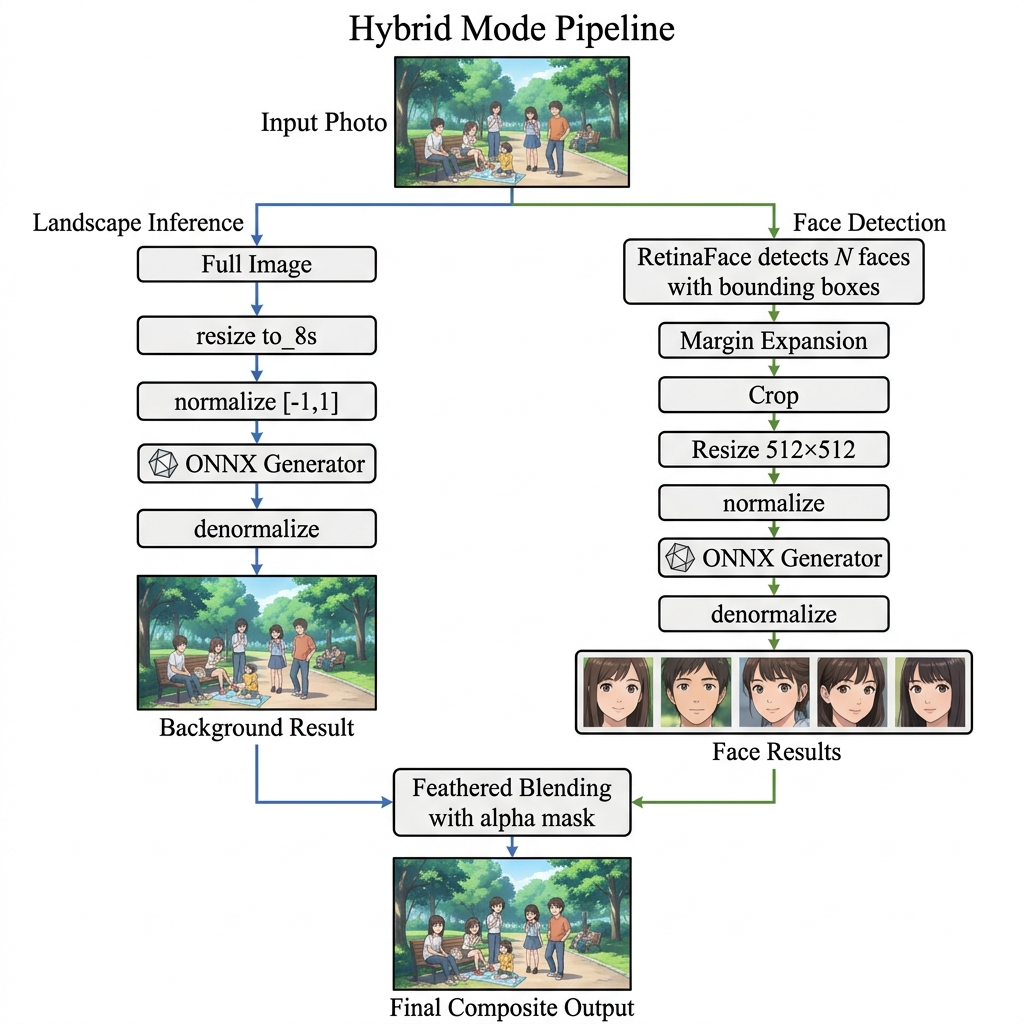
\includegraphics[width=0.95\textwidth]{figChap4/hybrid_mode_pipeline.png}
    \caption{Pipeline xử lý Hybrid Mode: kết hợp Landscape Inference cho nền và Face Inference cho từng khuôn mặt}
    \label{fig:hybrid_mode_pipeline}
\end{figure}

\begin{algorithm}[H]
\caption{Hybrid Mode --- kết hợp nền Landscape và khuôn mặt Face Mode}
\label{alg:hybrid_mode}
\begin{algorithmic}[1]
\Require Ảnh gốc $I$ kích thước $(H, W)$; mô hình ONNX $\mathcal{G}$; bộ phát hiện $\mathcal{D}$
\Ensure Ảnh anime $I_{\text{out}}$ kích thước $(H, W)$
\State $I_{\text{lim}}, s \gets \textsc{GiớiHạnCạnhDài}(I,\ 1280)$
\State $\mathcal{B} \gets \mathcal{D}(I_{\text{lim}})$ \Comment{danh sách bounding box}
\If{$\mathcal{B} = \varnothing$}
    \State \Return $\textsc{LandscapeMode}(I)$ \Comment{hạ cấp mềm}
\EndIf
\State $I_{\text{bg}} \gets \textsc{SuyLuận}(\mathcal{G},\ I)$ \Comment{Background Pass, giữ kích thước gốc}
\For{$b \in \mathcal{B}$}
    \State $b' \gets \textsc{MarginExpansion}(b)$ \Comment{Thuật toán~\ref{alg:margin_expansion}}
    \If{$\textsc{CạnhNhỏNhất}(b') < 16$}
        \State \textbf{chuyển sang khuôn mặt kế tiếp} \Comment{mặt quá nhỏ: giữ nguyên kết quả Landscape}
    \EndIf
    \State $C \gets \textsc{Cắt}(I_{\text{lim}},\ b')$; \quad $C \gets \textsc{Resize}(C,\ 512 \times 512)$
    \State $\widehat{C} \gets \textsc{SuyLuận}(\mathcal{G},\ C)$ \Comment{Face Pass}
    \State $b'_{\text{orig}} \gets b' / s$ \Comment{ánh xạ về hệ tọa độ ảnh gốc}
    \State $\widehat{C} \gets \textsc{Resize}(\widehat{C},\ w_f \times h_f)$ \Comment{$w_f, h_f$ suy từ $b'_{\text{orig}}$}
    \State $\delta \gets \textsc{TínhLề}(w_f,\ h_f)$ \Comment{Công thức~\eqref{eq:feather_margin}}
    \State $M \gets \textsc{TạoMặtNạViềnMờ}(w_f,\ h_f,\ \delta,\ \sigma = \delta/3)$
    \State $I_{\text{bg}} \gets \textsc{GhépAlpha}(I_{\text{bg}},\ \widehat{C},\ M,\ b'_{\text{orig}})$
\EndFor
\State \Return $I_{\text{bg}}$
\end{algorithmic}
\end{algorithm}

\subsection{Ánh xạ Tọa độ giữa Ảnh Giới hạn và Ảnh Gốc}
\label{subsec:hybrid_coord_mapping}

Do phát hiện khuôn mặt thực hiện trên ảnh đã giới hạn kích thước ($\leq 1280$ pixel), trong khi kết quả cuối cùng được ghép lên ảnh nền kích thước gốc $(W, H)$, hệ thống cần ánh xạ tọa độ bounding box từ không gian ảnh giới hạn sang không gian ảnh gốc:

\begin{equation}
\label{eq:hybrid_scale}
s = \begin{cases} \dfrac{1280}{\max(W, H)} & \text{nếu } \max(W, H) > 1280 \\[2ex] 1{,}0 & \text{ngược lại} \end{cases}
\end{equation}

Cho bounding box sau Margin Expansion $(x_1, y_1, x_2, y_2)$ trong ảnh giới hạn, tọa độ tương ứng trên ảnh gốc:
\begin{equation}
\label{eq:hybrid_map}
x_1^{\text{orig}} = \left\lfloor \frac{x_1}{s} + 0{,}5 \right\rfloor, \quad
y_1^{\text{orig}} = \left\lfloor \frac{y_1}{s} + 0{,}5 \right\rfloor, \quad
x_2^{\text{orig}} = \left\lfloor \frac{x_2}{s} + 0{,}5 \right\rfloor, \quad
y_2^{\text{orig}} = \left\lfloor \frac{y_2}{s} + 0{,}5 \right\rfloor
\end{equation}

\noindent trong đó biểu thức $\lfloor z + 0{,}5 \rfloor$ là phép làm tròn tới số nguyên gần nhất --- chính xác hơn phép cắt cụt $\lfloor z \rfloor$, vốn luôn thiên lệch về phía nhỏ hơn và tích lũy sai số dịch chuyển vùng ghép về góc trên bên trái.

Kích thước vùng mặt trên ảnh gốc:
\begin{equation}
\label{eq:hybrid_face_size}
w_f = \max(1,\; x_2^{\text{orig}} - x_1^{\text{orig}}), \quad
h_f = \max(1,\; y_2^{\text{orig}} - y_1^{\text{orig}})
\end{equation}

\noindent với toán tử $\max(1, \cdot)$ đảm bảo kích thước luôn hợp lệ, tránh lỗi chia cho 0 trong các phép resize tiếp theo khi bounding box suy biến.

Ảnh khuôn mặt sau suy luận (kích thước $512 \times 512$) được resize về $(w_f, h_f)$ bằng thuật toán nội suy Lanczos trước khi ghép. Lanczos được chọn thay vì bilinear vì nó dùng nhân lọc dựa trên hàm sinc, bảo toàn tốt hơn các thành phần tần số cao --- chính là những đường nét sắc mà toàn bộ pipeline đã nỗ lực tạo ra. Việc dùng một bộ nội suy làm mờ ở bước cuối sẽ triệt tiêu phần lớn lợi ích của các bước trước đó.

\medskip
\noindent\textit{\textbf{Nhận xét:} Bước ánh xạ tọa độ này là hệ quả trực tiếp của một quyết định thiết kế: phát hiện khuôn mặt trên ảnh đã thu nhỏ để tiết kiệm chi phí, nhưng dựng nền ở kích thước gốc để giữ chất lượng. Cái giá phải trả là sai số làm tròn: với ảnh 4000~pixel thu về 1280 ($s = 0{,}32$), mỗi pixel sai lệch trong không gian phát hiện tương ứng khoảng 3~pixel trong ảnh gốc. Sai số này không ảnh hưởng tới chất lượng khuôn mặt được sinh ra, nhưng làm vùng ghép có thể lệch vài pixel so với vị trí lý tưởng. Kỹ thuật feathered blending ở mục tiếp theo, với vùng chuyển tiếp rộng $2\delta$ ---~tức khoảng $16\%$ cạnh nhỏ của vùng mặt~---, đủ sức che lấp mức lệch này --- một ví dụ cho thấy hai thành phần trong pipeline có thể bù trừ lẫn nhau, và việc phân tích chúng tách rời sẽ bỏ sót mối quan hệ đó.}

\subsection{Kỹ thuật Feathered Blending}
\label{subsec:feathered_blending}

Khi ghép trực tiếp vùng mặt (xử lý Face Mode ở $512 \times 512$) vào nền (xử lý Landscape ở độ phân giải khác), sẽ xuất hiện đường biên rõ ràng do khác biệt về phong cách và độ phân giải giữa hai vùng. Kỹ thuật \textbf{feathered blending} sử dụng mặt nạ alpha với viền mờ Gaussian để tạo vùng chuyển tiếp mượt mà.

\begin{figure}[H]
    \centering
    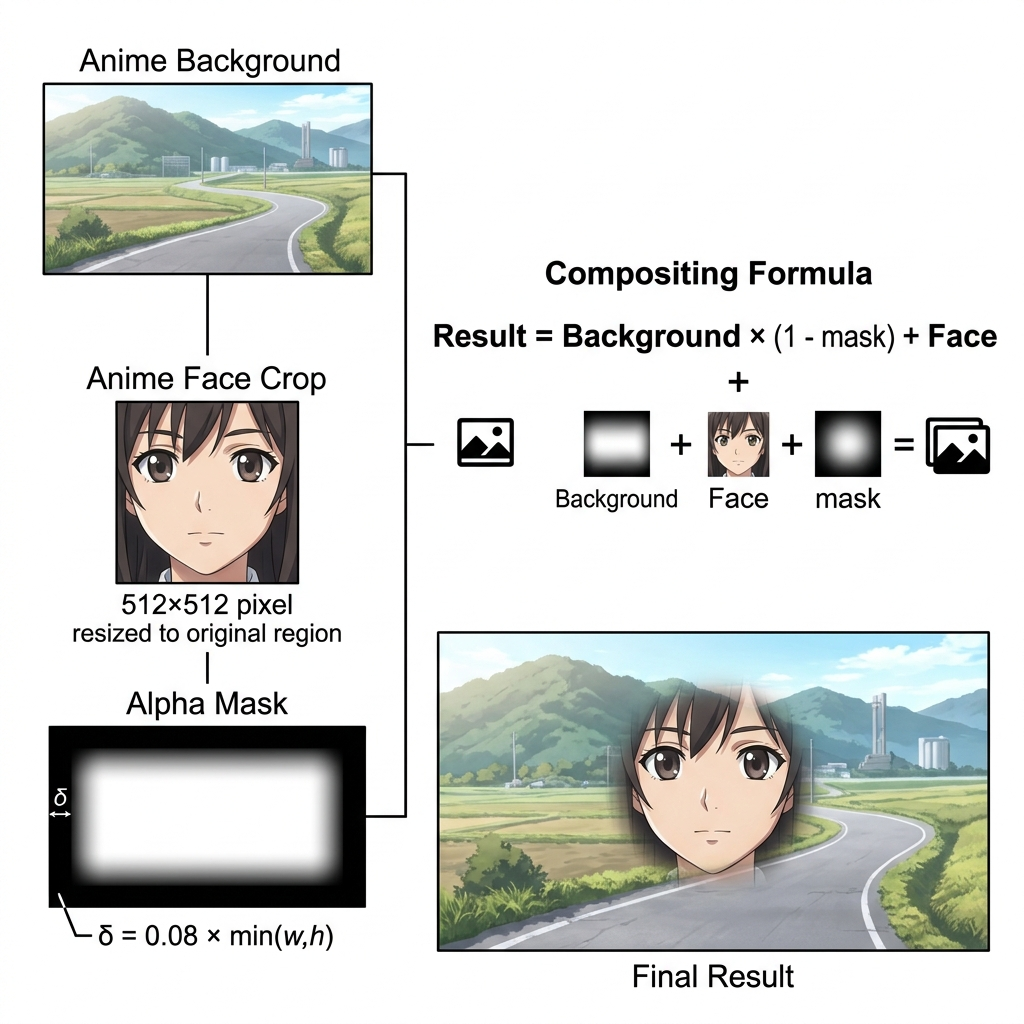
\includegraphics[width=0.85\textwidth]{figChap4/feathered_blending.png}
    \caption{Kỹ thuật Feathered Blending: mặt nạ alpha với viền mờ Gaussian tạo vùng chuyển tiếp liền mạch}
    \label{fig:feathered_blending}
\end{figure}

Quy trình tạo mặt nạ alpha gồm 3 bước:

\textbf{Bước 1 --- Tạo mặt nạ nền đen:} Khởi tạo ảnh grayscale kích thước $(w_f, h_f)$ với tất cả pixel có giá trị 0:
\begin{equation}
\label{eq:mask_init}
M(x, y) = 0 \quad \forall\; (x, y) \in [0, w_f) \times [0, h_f)
\end{equation}

\textbf{Bước 2 --- Vẽ vùng trắng thu nhỏ:} Vẽ hình chữ nhật trắng (giá trị 255) bên trong mặt nạ, thu nhỏ mỗi cạnh một lề $\delta$:
\begin{equation}
\label{eq:feather_margin}
\begin{aligned}
m &= \min(w_f, h_f), \qquad \delta_0 = \lfloor 0{,}08\, m \rfloor, \\[2pt]
\delta &= \min\!\left( \max(\delta_0,\ \delta_{\min}),\ \left\lfloor \tfrac{m-1}{4} \right\rfloor \right), \qquad \delta_{\min} = 3
\end{aligned}
\end{equation}
\begin{equation}
\label{eq:mask_rect}
M(x, y) = \begin{cases} 255 & \text{nếu } \delta \leq x < w_f - \delta \text{ và } \delta \leq y < h_f - \delta \\ 0 & \text{ngược lại} \end{cases}
\end{equation}

Hai phép chặn trong Công thức~\eqref{eq:feather_margin} tồn tại để xử lý các trường hợp suy biến khi khuôn mặt quá nhỏ. \textbf{Chặn dưới} $\delta_{\min} = 3$ giữ cho dải chuyển tiếp đủ rộng để mắt người không nhận ra ranh giới; nếu để $\delta$ tỉ lệ thuần theo $8\%$, một vùng mặt $20$~pixel sẽ chỉ có lề $1$~pixel --- tương đương ghép cứng. \textbf{Chặn trên} $\lfloor (m-1)/4 \rfloor$ bảo đảm vùng lõi bão hòa của mặt nạ luôn chiếm ít nhất một nửa cạnh nhỏ. Thiếu chặn này, khi $m < 2\delta_{\min} + 1 = 7$ thì hai lề trái và phải gặp nhau, hình chữ nhật trắng suy biến thành một đường thẳng hoặc rỗng: mặt nạ trở thành toàn 0 và khuôn mặt đã phong cách hóa bị loại bỏ hoàn toàn khỏi ảnh kết quả mà hệ thống không báo lỗi. Chặn trên chỉ có hiệu lực khi $m < 13$, nên không làm thay đổi bất kỳ kết quả thực nghiệm nào trong luận văn. Ở tầng cao hơn, hệ thống còn bỏ qua nhánh Face Mode khi $\min(w_f, h_f) < 16$ (Thuật toán~\ref{alg:hybrid_mode}), vì việc phóng một vùng cắt nhỏ như vậy lên $512 \times 512$ không bổ sung được chi tiết nào so với nhánh Landscape.

\textbf{Bước 3 --- Làm mờ Gaussian:} Áp dụng bộ lọc Gaussian Blur với \textit{độ lệch chuẩn} $\sigma = \delta/3$ lên mặt nạ, tạo vùng chuyển tiếp gradient từ 255 (trung tâm) về 0 (biên):
\begin{equation}
\label{eq:gaussian_blur}
\hat{M} = M * G_\sigma, \qquad \sigma = \frac{\delta}{3}, \qquad G_\sigma(x,y) = \frac{1}{2\pi\sigma^2}\, e^{-\frac{x^2+y^2}{2\sigma^2}}
\end{equation}

Phép ghép cuối cùng sử dụng alpha compositing theo mặt nạ $\hat{M}$:
\begin{equation}
\label{eq:alpha_composite}
I_{\text{out}}(x,y) = \underbrace{\frac{\hat{M}(x,y)}{255}}_{\alpha(x,y)} \cdot I_{\text{face}}(x,y) + \left(1 - \frac{\hat{M}(x,y)}{255}\right) \cdot I_{\text{bg}}(x,y)
\end{equation}

\noindent trong đó $I_{\text{face}}$ là ảnh khuôn mặt đã suy luận (resize về $w_f \times h_f$), $I_{\text{bg}}$ là ảnh nền anime tại vùng $(x_1^{\text{orig}}, y_1^{\text{orig}})$, và $\alpha(x,y) \in [0,1]$ là hệ số pha trộn.

\textbf{Phân tích cơ chế.} Ba bước trên phối hợp tạo ra một hàm $\alpha$ có ba vùng rõ rệt:
\begin{itemize}
    \item \textbf{Vùng lõi} (cách biên từ $2\delta$ trở vào): $\alpha = 1$ ---~đúng bằng 1 chứ không phải xấp xỉ, và đúng cả tại bốn góc~---, ảnh đầu ra lấy hoàn toàn từ khuôn mặt chất lượng cao.
    \item \textbf{Vùng chuyển tiếp} (dải rộng khoảng $2\delta$ quanh biên hình chữ nhật trong): $\alpha$ biến thiên trơn từ 1 xuống 0 theo dạng hàm lỗi (tích phân của Gaussian).
    \item \textbf{Vùng ngoài cùng} (sát mép hình dán): $\alpha < 10^{-3}$, ảnh đầu ra lấy hoàn toàn từ nền; nói cách khác phép ghép không làm thay đổi một pixel nào của ảnh nền bên ngoài vùng cắt.
\end{itemize}

\textbf{Ràng buộc $\sigma = \delta/3$: áp dụng quy tắc 3-sigma cho vùng chuyển tiếp.} Việc thu hình chữ nhật trắng vào trong một lề $\delta$ \textit{trước khi} làm mờ là chi tiết then chốt, nhưng chỉ phát huy tác dụng nếu bán kính làm mờ được chọn tương thích với lề đó. Nếu vẽ hình chữ nhật trắng phủ kín rồi mới làm mờ, giá trị $\alpha$ tại mép ngoài sẽ là $0{,}5$ chứ không phải 0 --- đường biên cứng vẫn hiện ra, chỉ mờ hơn. Ngược lại, nếu thu vào lề $\delta$ nhưng lấy bán kính làm mờ cũng bằng $\delta$ thì đuôi Gaussian \textit{chưa} tắt khi chạm mép ngoài, vì $\delta$ chỉ tương ứng $1\sigma$.

Luận văn ràng buộc hai tham số theo \textbf{quy tắc 3-sigma}: đặt $\sigma = \delta/3$ thì hơn $99{,}7\%$ khối lượng của nhân Gaussian nằm trong khoảng $\pm 3\sigma = \pm\delta$ quanh cạnh của hình chữ nhật trắng. Toàn bộ đoạn dốc của hàm $\alpha$ vì thế nằm trọn trong dải lề, trải trên bề rộng đúng bằng $2\delta$, và kéo theo hai tính chất mà phiên bản $\sigma = \delta$ không có:

\begin{enumerate}
    \item \textbf{Bảo toàn nền tại mép dán.} Tại pixel ngoài cùng của hình chữ nhật dán, $\alpha \to 0$, nên $I_{\text{out}} = I_{\text{bg}}$ trong phạm vi một bước lượng tử hóa. Đường biên bị \textit{khử} chứ không chỉ bị làm nhạt.
    \item \textbf{Bảo toàn chi tiết khuôn mặt.} Ở độ sâu $2\delta$ trở vào, $\hat{M} = 255$ trên toàn bộ vùng lõi, \textit{kể cả bốn góc}. Đây là điểm mà lựa chọn $\sigma = \delta$ thất bại: gần góc, hai đáp ứng cạnh trực giao nhân với nhau nên $\alpha$ chỉ đạt khoảng $0{,}70$, làm khuôn mặt bị pha loãng $30\%$ tại bốn góc vùng cắt.
\end{enumerate}

Bảng~\ref{tab:sigma_choice} đối chiếu hai lựa chọn, số liệu đo trực tiếp trên mặt nạ do chương trình sinh ra với vùng mặt $512 \times 512$ ($\delta = 40$).

\begin{table}[H]
\caption{Ảnh hưởng của bán kính làm mờ tới chất lượng mặt nạ alpha}
\label{tab:sigma_choice}
\centering
\begin{tabular}{|c|c|c|c|}
\hline
\textbf{Lựa chọn} & \textbf{$\alpha$ tại mép dán} & \textbf{$\alpha$ tại góc, sâu $2\delta$} & \textbf{Hệ quả thị giác} \\
\hline
$\sigma = \delta$ & $0{,}185$ & $0{,}70$ & Còn bậc nhảy ở biên, mờ góc \\
\hline
$\sigma = \delta/3$ & $< 10^{-3}$ & $1{,}00$ & Liền mạch, giữ nguyên chi tiết \\
\hline
\end{tabular}
\end{table}

Một hệ quả thực dụng của ràng buộc này là hai tham số được tách vai trò rõ ràng: $\sigma$ bị khóa theo $\delta$ và không cần tinh chỉnh, còn $\delta$ trở thành tham số cảm quan duy nhất, quyết định bề rộng dải hòa trộn. Hệ số $\delta = 8\%$ cạnh nhỏ hơn của vùng mặt được chọn qua thực nghiệm: nhỏ hơn sẽ tạo đường viền rõ, lớn hơn sẽ làm mờ quá nhiều chi tiết khuôn mặt.

\medskip
\noindent\textit{\textbf{Nhận xét phản biện:} Feathered blending là giải pháp đơn giản và rẻ, nhưng có ba hạn chế mà luận văn cho rằng cần nêu rõ. \textbf{Thứ nhất, mặt nạ có dạng hình chữ nhật chứ không bám theo đường viền khuôn mặt.} Hệ quả là vùng chuyển tiếp cắt ngang qua tóc, vai và nền một cách tùy tiện; ở những nơi này, ảnh đầu ra là trung bình có trọng số của hai phiên bản anime hóa \textit{khác nhau} của cùng một nội dung, có thể gây hiện tượng chồng mờ nhẹ. \textbf{Thứ hai, alpha blending không hiệu chỉnh chênh lệch tông màu.} Nếu hai lần suy luận cho ra tông sáng khác biệt --- điều hoàn toàn có thể xảy ra vì LADE tính thống kê chuẩn hóa trên toàn ảnh, mà hai đầu vào có nội dung khác nhau --- thì phép trung bình chỉ làm mềm ranh giới chứ không xóa được sự chênh lệch. Kỹ thuật Poisson Image Editing \cite{Perez2003Poisson}, giải phương trình Poisson với điều kiện biên Dirichlet để bảo toàn gradient của vùng ghép trong khi khớp giá trị tuyệt đối tại biên, giải quyết đúng vấn đề này và được đề xuất ở Chương~5. \textbf{Thứ ba, tỉ lệ $\delta = 8\%$ là hằng số duy nhất cho mọi ảnh.} Hai phép chặn trong Công thức~\eqref{eq:feather_margin} chỉ can thiệp ở chế độ suy biến (khuôn mặt rất nhỏ) chứ không thích ứng theo nội dung; trong khi đó mức chênh lệch giữa hai lần suy luận lại thay đổi theo từng ảnh --- một cơ chế điều chỉnh $\delta$ thích ứng theo độ lệch tông màu đo được sẽ hợp lý hơn. Mặc dù vậy, cần đặt các hạn chế này trong đúng bối cảnh: kết quả khảo sát người dùng ở Chương~4 cho thấy phần lớn người tham gia ưu tiên đầu ra Hybrid Mode, nên giải pháp hiện tại đã đủ tốt cho mục tiêu ứng dụng --- các cải tiến nêu trên thuộc loại tinh chỉnh chứ không phải sửa lỗi.}

\subsection{Phân tích Độ phức tạp}
\label{subsec:hybrid_complexity}

Gọi $T_L$ là thời gian suy luận Landscape, $T_F$ là thời gian suy luận Face ($512 \times 512$), $T_D$ là thời gian phát hiện mặt, $T_{\text{blend}}$ là thời gian tạo mặt nạ và ghép, $N$ là số khuôn mặt phát hiện được. Tổng thời gian xử lý Hybrid Mode:

\begin{equation}
\label{eq:hybrid_time}
T_{\text{hybrid}} = T_D + T_L + N \cdot \left(T_F + T_{\text{blend}}\right)
\end{equation}

\noindent trong đó $T_{\text{blend}} \ll T_F$ (tạo mask và ghép ảnh là các phép toán trên mảng, rất nhanh so với suy luận mạng nơ-ron). So sánh với các chế độ khác:

\begin{table}[H]
\caption{Phân tích độ phức tạp thời gian giữa ba chế độ}
\label{tab:mode_complexity}
\centering
\begin{tabular}{|l|c|c|}
\hline
\textbf{Chế độ} & \textbf{Số lần suy luận ONNX} & \textbf{Tổng thời gian} \\
\hline
Face Mode & 1 & $T_D + T_F$ \\
\hline
Landscape Mode & 1 & $T_L$ \\
\hline
Hybrid Mode & $1 + N$ & $T_D + T_L + N \cdot T_F$ \\
\hline
\end{tabular}
\end{table}

Chi phí tính toán của Hybrid Mode tăng \textbf{tuyến tính} theo số khuôn mặt. Tuy nhiên, do $T_F$ sử dụng kích thước đầu vào cố định $512 \times 512$ --- thường nhỏ hơn ảnh Landscape --- thời gian mỗi lần suy luận Face thường nhanh hơn suy luận Landscape. Trong thực nghiệm (Chương~4), ảnh có 2--3 khuôn mặt thường hoàn thành Hybrid Mode trong thời gian chấp nhận được cho ứng dụng tương tác.

\textbf{Hướng tối ưu hóa khả thi.} Do $N$ lần suy luận khuôn mặt hoàn toàn độc lập với nhau, chúng có thể được gộp thành \textbf{một lần suy luận theo lô} (batch inference) với tensor đầu vào kích thước $N \times 3 \times 512 \times 512$. Trên GPU, chi phí của một lô $N$ ảnh nhỏ hơn nhiều so với $N$ lần chạy riêng lẻ, vì phần lớn thời gian của mỗi lần chạy riêng là chi phí cố định (khởi động kernel, truyền dữ liệu) chứ không phải tính toán thực sự. Cải tiến này sẽ biến thành phần $N \cdot T_F$ thành gần như hằng số với $N$ nhỏ, và được khuyến nghị cho phiên bản tiếp theo.

% =====================================================
\section{Phân tích Kỹ thuật và Đánh giá Thiết kế}
\label{sec:fe_analysis}

\subsection{Lý do Chọn RetinaFace MobileNet 0.25}
\label{subsec:why_retinaface}

So với các phương pháp phát hiện khuôn mặt phổ biến khác, RetinaFace với backbone MobileNet 0.25 có ưu thế rõ ràng trong bối cảnh triển khai thực tế:

\begin{table}[H]
\caption{So sánh các phương pháp phát hiện khuôn mặt cho ứng dụng thực tế}
\label{tab:face_det_comparison}
\centering
\begin{tabular}{|p{3cm}|p{2cm}|p{2.5cm}|p{2.5cm}|p{2.5cm}|}
\hline
\textbf{Phương pháp} & \textbf{Tốc độ} & \textbf{Landmark} & \textbf{Multi-scale} & \textbf{Model size} \\
\hline
Viola-Jones \cite{ViolaJones2004} & Rất nhanh & Không & Có hạn & Nhỏ \\
\hline
MTCNN \cite{Zhang2016MTCNN} & Trung bình & 5 điểm & Tốt & Nhỏ \\
\hline
SSD Face \cite{Liu2016SSD} & Nhanh & Không & Tốt & Trung bình \\
\hline
\textbf{RetinaFace MN0.25} \cite{Deng2019RetinaFace} & \textbf{Nhanh} & \textbf{5 điểm} & \textbf{Rất tốt} & \textbf{Rất nhỏ} \\
\hline
RetinaFace ResNet50 & Chậm & 5 điểm & Xuất sắc & Lớn \\
\hline
\end{tabular}
\end{table}

Các lý do kỹ thuật cụ thể:
\begin{itemize}
    \item \textbf{Tương thích ONNX Runtime:} RetinaFace được xuất sang ONNX một cách tự nhiên, dùng chung runtime với AnimeGANv3. Hệ thống vì vậy chỉ cần một thư viện suy luận duy nhất --- giảm đáng kể độ phức tạp triển khai và kích thước gói cài đặt.
    \item \textbf{5 facial landmarks:} Thông tin landmarks được sử dụng trong Margin Expansion của Hybrid Mode để dịch chuyển vùng cắt theo hướng mặt, và còn mở ra khả năng face alignment trong các phiên bản tương lai.
    \item \textbf{Multi-scale FPN:} Phát hiện tốt cả khuôn mặt nhỏ trong ảnh góc rộng lẫn khuôn mặt lớn trong ảnh cận cảnh --- yêu cầu bắt buộc với Hybrid Mode xử lý ảnh nhóm.
    \item \textbf{Kích thước model nhỏ ($\sim$500~KB):} Cùng với model AnimeGANv3 9,1~MB, tổng dung lượng hệ thống dưới 10~MB --- phù hợp để đóng gói vào file thực thi hoặc tải về trong ứng dụng web.
\end{itemize}

\textbf{Vì sao không chọn MTCNN?} MTCNN cũng cung cấp 5 landmark với kích thước mô hình nhỏ, nhưng dùng kiến trúc ba tầng nối tiếp (P-Net, R-Net, O-Net) hoạt động trên kim tự tháp ảnh. Cách này khiến thời gian xử lý \textit{phụ thuộc vào số lượng ứng viên} phát sinh ở mỗi tầng, gây biến động lớn giữa các ảnh --- đặc tính bất lợi cho một dịch vụ web cần thời gian phản hồi ổn định. RetinaFace là mô hình một lượt, chi phí gần như cố định theo kích thước ảnh.

\subsection{Đánh giá Pipeline Tổng thể}
\label{subsec:pipeline_evaluation}

Pipeline được thiết kế theo nguyên tắc \textbf{hạ cấp mềm} (graceful degradation): nếu không phát hiện được khuôn mặt (confidence dưới ngưỡng 0,8, hoặc khuôn mặt bị che khuất), hệ thống tự động chuyển sang chế độ Landscape để xử lý toàn bộ ảnh, tránh trả về lỗi cho người dùng. Cơ chế này áp dụng cho cả Face Mode lẫn Hybrid Mode.

Bảng~\ref{tab:face_vs_landscape} tóm tắt sự đánh đổi giữa ba chế độ. Face Mode cho chất lượng anime cao nhất đối với ảnh chân dung do ba cơ chế đã phân tích ở Mục~\ref{subsec:eff_res_discussion}: chuẩn hóa độ phân giải khuôn mặt về khoảng 286~pixel (bề rộng hiệu dụng khi dùng đầu vào $512\times512$ với $m = 0{,}3$ trên thang tham chiếu $\max(\cdot)$), tập trung toàn bộ năng lực Generator vào khuôn mặt, và loại bỏ ảnh hưởng của nền lên các cơ chế thống kê toàn cục.

Hybrid Mode khắc phục nhược điểm mất nền của Face Mode bằng cách xử lý riêng từng khu vực, đổi lại chi phí tính toán tăng tuyến tính theo số khuôn mặt.

\subsection{Hạn chế của Thiết kế}
\label{subsec:pipeline_limitations}

Để đánh giá cân bằng, cần chỉ rõ những hạn chế nội tại của pipeline --- ngoài các hạn chế cục bộ đã nêu ở từng mục:

\begin{enumerate}
    \item \textbf{Sai sót lan truyền một chiều.} Hai mô hình mắc nối tiếp mà không có cơ chế phản hồi: nếu RetinaFace trả về bounding box lệch (thường gặp ở góc nghiêng $> 60°$), Generator sẽ xử lý một vùng cắt sai và không có cách nào phát hiện điều đó. Không tồn tại bước kiểm tra chất lượng nào giữa hai giai đoạn.
    \item \textbf{Vùng cắt không vuông gây biến dạng.} Như đã nêu ở Tính chất 2 (Mục~\ref{subsec:margin_properties}), khuôn mặt gần biên trên/dưới cho vùng cắt hình chữ nhật, và phép resize về $512\times512$ làm biến dạng tỉ lệ. Giải pháp là đệm viền bằng màu trung bình hoặc phản chiếu gương thay vì cắt cụt.
    \item \textbf{Landmarks chưa được khai thác đầy đủ.} Năm điểm đặc trưng sẵn có hiện được AGME dùng để ước lượng góc xoay và dịch chuyển lề, nhưng chưa được khai thác cho căn chỉnh khuôn mặt (face alignment) theo góc nghiêng trong mặt phẳng ảnh --- bỏ lỡ cơ hội cải thiện đúng nhóm ảnh khó nhất.
    \item \textbf{Chọn chế độ thủ công.} Người dùng phải tự chọn chế độ, trong khi phân tích ở Mục~\ref{sec:effective_resolution} cho thấy hoàn toàn có thể chọn tự động dựa trên tỉ lệ kích thước khuôn mặt.
    \item \textbf{Không có nhất quán thời gian.} Khi xử lý video, mỗi khung hình được phát hiện và cắt độc lập; bounding box dao động nhẹ giữa các khung hình liên tiếp sẽ khuếch đại thành hiện tượng nhấp nháy ở đầu ra. Vấn đề này được bàn tiếp ở Chương~5.
\end{enumerate}

\subsection{Cân nhắc về Quyền riêng tư}
\label{subsec:privacy}

Do hệ thống xử lý ảnh khuôn mặt --- một dạng dữ liệu sinh trắc học --- luận văn ghi nhận một số nguyên tắc đã được áp dụng trong quá trình triển khai. Toàn bộ quá trình phát hiện và chuyển đổi diễn ra trong một lần gọi API duy nhất; ảnh đầu vào không được lưu trữ lâu dài trên máy chủ sau khi trả kết quả, và hệ thống không thực hiện bất kỳ thao tác nhận dạng hay đối sánh danh tính nào --- RetinaFace chỉ được dùng để \textit{định vị} khuôn mặt, không phải để \textit{nhận diện} người. Các ảnh sử dụng trong phần đánh giá định tính ở Chương~4 đều thuộc nhóm ảnh công khai hoặc có sự đồng ý của người trong ảnh. Với một hệ thống có khả năng sinh ảnh chân dung biến đổi, luận văn cũng lưu ý rằng việc sử dụng cần tuân thủ nguyên tắc không tạo nội dung gây hiểu nhầm về danh tính hoặc gây tổn hại đến người được chụp.

\medskip
\noindent\textit{\textbf{Thảo luận:} Nhìn lại toàn chương, đóng góp của luận văn có thể tóm gọn trong một câu: \textbf{thay vì dạy mô hình chú ý tới khuôn mặt, hãy chỉ đưa khuôn mặt cho mô hình xem}. Cách tiếp cận này có ưu điểm rõ ràng --- không cần huấn luyện lại, tái sử dụng được mọi mô hình phong cách, mỗi thành phần nâng cấp độc lập --- nhưng cũng bộc lộ giới hạn của kiến trúc kiểu ống dẫn: các giai đoạn không thể học từ nhau, và mỗi giai đoạn tối ưu cho mục tiêu riêng của nó chứ không phải cho chất lượng cuối cùng. Một hệ thống huấn luyện đầu-cuối, trong đó tín hiệu về chất lượng ảnh anime có thể truyền ngược tới tận khâu chọn vùng cắt, về lý thuyết sẽ cho kết quả tốt hơn. Nhưng nó cũng sẽ đắt hơn nhiều lần về dữ liệu và tính toán, đồng thời đánh mất tính mô-đun --- thứ tài sản quý nhất của giải pháp hiện tại. Trong bối cảnh một luận văn hướng tới hệ thống chạy được trên tài nguyên hạn chế, luận văn cho rằng đánh đổi này là hợp lý, và ghi nhận hướng đầu-cuối như một triển vọng nghiên cứu chứ không phải một thiếu sót cần khắc phục ngay.}

\section*{Tổng kết chương}

Chương này đã trình bày luồng xử lý anime tích hợp phát hiện khuôn mặt --- đóng góp kỹ thuật cốt lõi của luận văn:

\begin{itemize}
    \item \textbf{Nguyên tắc thiết kế:} Can thiệp ở tầng pipeline thay vì sửa kiến trúc hay hàm mất mát của DTGAN, qua đó giữ nguyên mô hình đã huấn luyện và bảo toàn tính mô-đun của hệ thống.
    \item \textbf{Pipeline end-to-end} tích hợp ba chế độ Face Mode, Landscape Mode và Hybrid Mode, với cơ chế hạ cấp mềm tự động chuyển chế độ khi không phát hiện khuôn mặt.
    \item \textbf{Luồng dữ liệu qua RetinaFace:} tiền xử lý chuẩn ImageNet $\to$ backbone MobileNet~0.25 (tiết kiệm $\approx 9\times$ chi phí nhờ depthwise separable convolution) $\to$ FPN đa tỉ lệ $\to$ giải mã Prior Box $\to$ lọc ngưỡng $\to$ NMS $\to$ sắp xếp theo diện tích. Bộ tham số $(0{,}8;\ 0{,}3;\ 10;\ 5)$ thể hiện nhất quán triết lý ưu tiên độ chính xác hơn độ bao phủ, phù hợp với hậu quả bất đối xứng của hai loại lỗi.
    \item \textbf{Thuật toán AGME} 6 bước (Thuật toán~\ref{alg:margin_expansion}): neo lề vào thang tham chiếu $w = \max(\cdot)$ để lượng ngữ cảnh không co lại ở tư thế nghiêng, ước lượng hệ số dịch chuyển $S$ từ bất đối xứng mũi--mắt rồi phân bổ lại ngân sách cố định $2mw$ thành $m(1-S)w$ và $m(1+S)w$, chia phần dư thừa dọc theo tỉ lệ $70{:}30$, duy trì tỉ lệ 1:1 và xử lý phân nhánh khi $dy < 0$. Tính chất quan trọng nhất được rút ra: với $m = 0{,}3$ và đầu vào $512 \times 512$, khuôn mặt luôn được đưa vào Generator ở bề rộng \textbf{ít nhất 256 pixel} (điển hình $\approx 286$), không phụ thuộc kích thước ảnh gốc.
    \item \textbf{Phân tích độ phân giải hiệu dụng:} Hệ số lợi ích $\kappa = 256/(s \cdot w)$ cho thấy Face Mode mang lại lợi ích về độ phân giải khi khuôn mặt hẹp hơn 256~pixel trong ảnh đã giới hạn kích thước, và lợi ích lớn nhất ở ảnh nhóm hoặc ảnh chụp xa. Hai cơ chế bổ sung --- khớp phân phối huấn luyện và loại bỏ nhiễu nền --- đóng góp độc lập với kích thước khuôn mặt.
    \item \textbf{Hybrid Mode với Feathered Blending} (Thuật toán~\ref{alg:hybrid_mode}): xử lý nền Landscape và từng khuôn mặt Face Mode riêng biệt, ghép bằng mặt nạ alpha làm mờ Gaussian với lề $\delta = 8\%$ và bán kính làm mờ ràng buộc theo quy tắc 3-sigma ($\sigma = \delta/3$), kèm hai phép chặn giá trị $\delta$ để an toàn với khuôn mặt nhỏ. Chi phí tăng tuyến tính theo số khuôn mặt, có thể tối ưu bằng suy luận theo lô.
\end{itemize}

Chương cũng đã chỉ rõ các hạn chế của thiết kế: sai sót lan truyền một chiều giữa hai mô hình nối tiếp, vùng cắt không vuông ở biên ảnh, landmark chưa được khai thác cho căn chỉnh khuôn mặt, và mặt nạ ghép có dạng hình chữ nhật thay vì bám theo đường viền khuôn mặt.

Chương~4 tiếp theo sẽ kiểm chứng bằng thực nghiệm các phân tích lý thuyết đã trình bày: đánh giá độ chính xác phát hiện khuôn mặt theo từng kịch bản, khảo sát ảnh hưởng của tham số $m$ tới chất lượng đầu ra, so sánh định lượng và định tính giữa ba chế độ, cùng đánh giá cảm nhận từ người dùng thực tế.